\chapter{Background Estimation}

\section{Irreducible Backgrounds}
\label{sec:irrbkgd}

\subsection{\qqZZ~ Modelling}
\label{sec:redbkgd}

The \qqZZ~ background is generated at NLO, while the fully differential cross section has been computed at 
NNLO~\cite{Grazzini2015407}, but are not yet available in a partonic level event generator. Therefore NNLO/NLO 
$k$-factors for the \qqZZ~background process are applied to the {\sc powheg} sample. The inclusive cross 
sections obtained using the same PDF and renormalization and factorization scales as the {\sc powheg} sample
at LO, NLO, and NNLO are shown in Table~\ref{tab:qqZZXS}. The NNLO/NLO $k$-factors are applied in the analysis
differentally as a function of $m(\cPZ\cPZ)$. 

Additional NLO electroweak corrections which depend on the initial state quark flavor and kinematics
are also applied to the \qqZZ~ background process in the region $m(\cPZ \cPZ)>2m(\cPZ)$ where the 
corrections have been computed. The differential QCD and electroweak $k$-factors can be seen in 
Figure~\ref{fig:qqZZKfactor}.

\begin{table}[h]
    \centering
    \begin{tabular}{|l|c|c|} 
\hline %----------------------------------------------------------------
QCD Order  & $\sigma_{2\ell2\ell^{\prime}} (\mathrm{fb})$  & $\sigma_{4\ell} (\mathrm{fb})$  \\
\hline %----------------------------------------------------------------
LO    & 218.5$^{+16\%}_{-15\%}$ & 98.4$^{+13\%}_{-13\%}$ \\
NLO   & 290.7$^{+5\%}_{-8\%}$   & 129.5$^{+4\%}_{-6\%}$ \\
NNLO  & 324.0$^{+2\%}_{-3\%}$   & 141.2$^{+2\%}_{-2\%}$ \\
\hline %----------------------------------------------------------------
    \end{tabular}
    \caption{Cross sections for \qqZZ~ production at 13 \TeV}
    \label{tab:qqZZXS}
\end{table}

%=======
\begin{figure}[!htb]
\vspace*{0.3cm}
\begin{center}
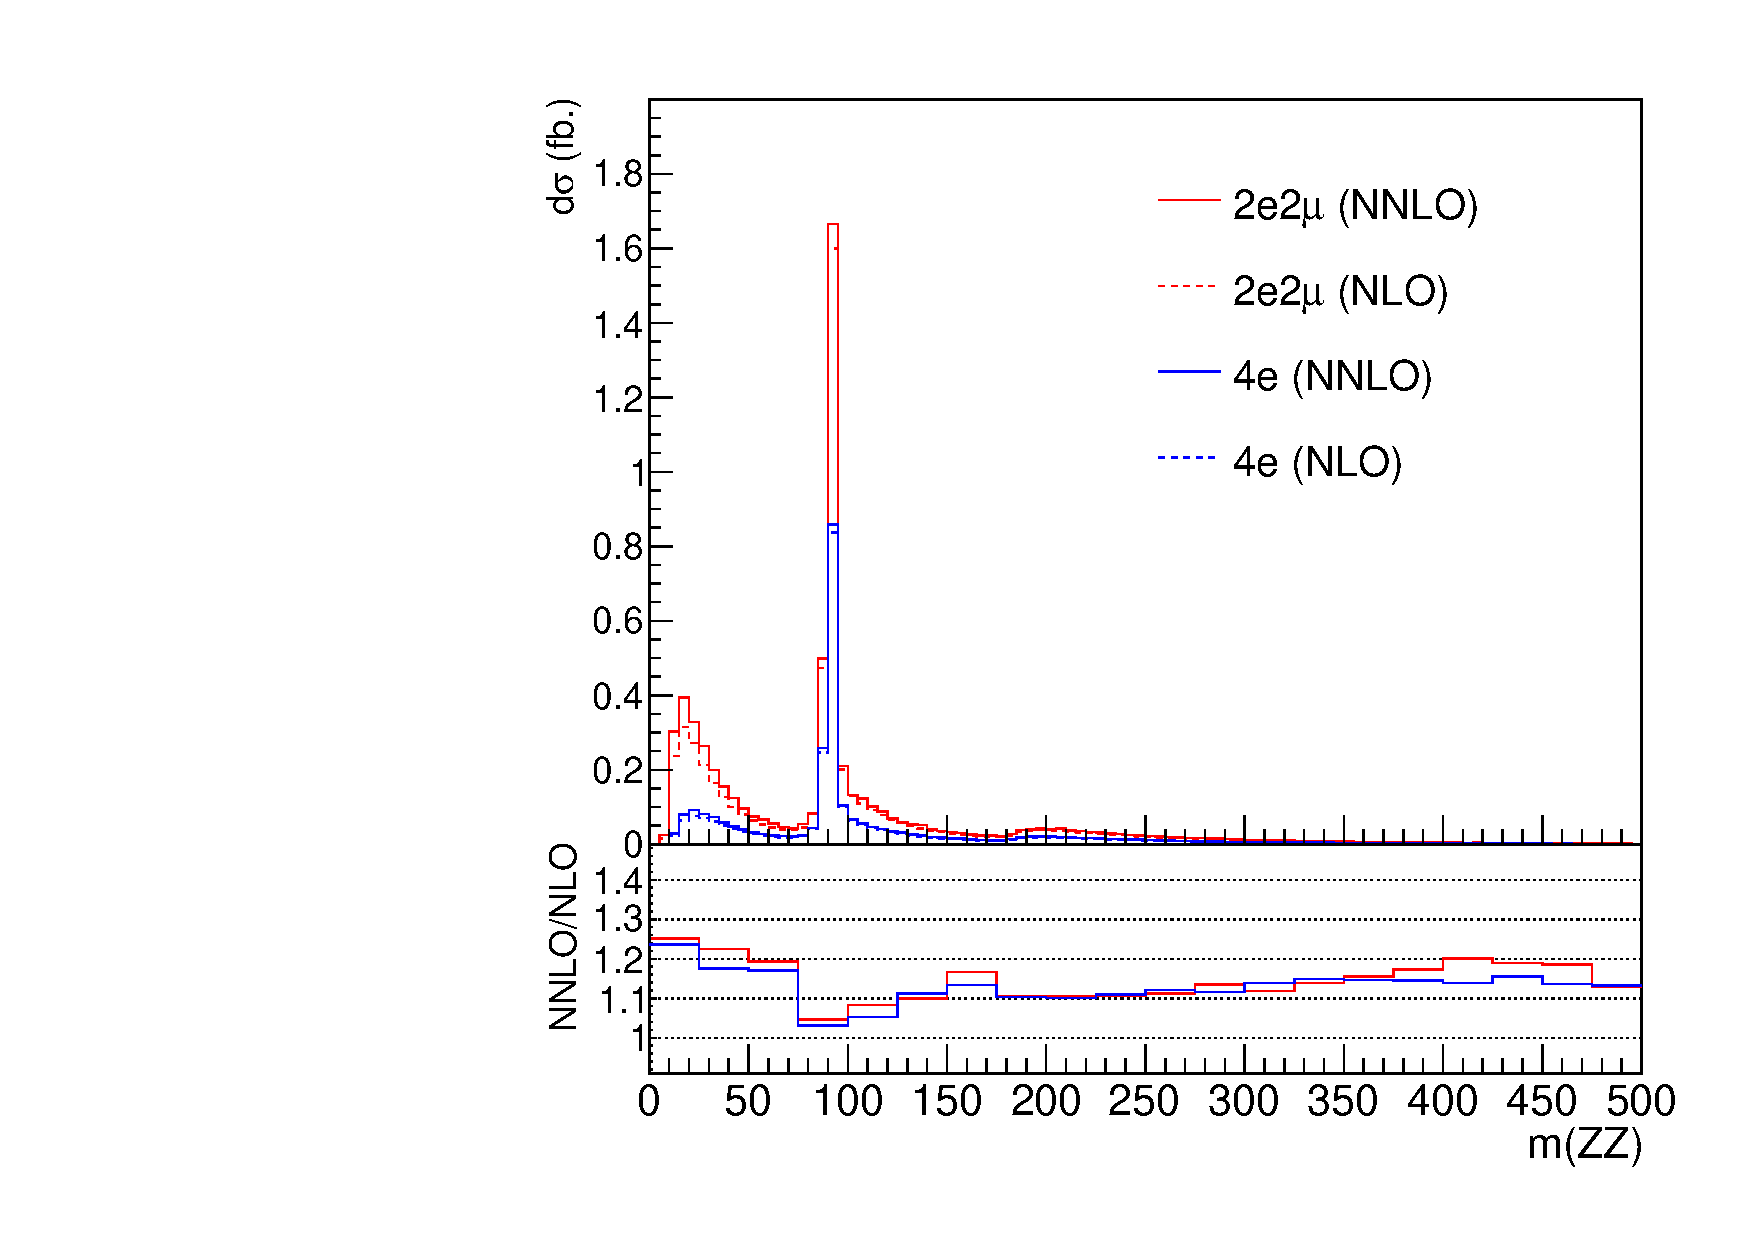
\includegraphics[width=0.48\textwidth]{Figures/IrrBkg/Kfactor_qqZZ_mZZ.pdf}
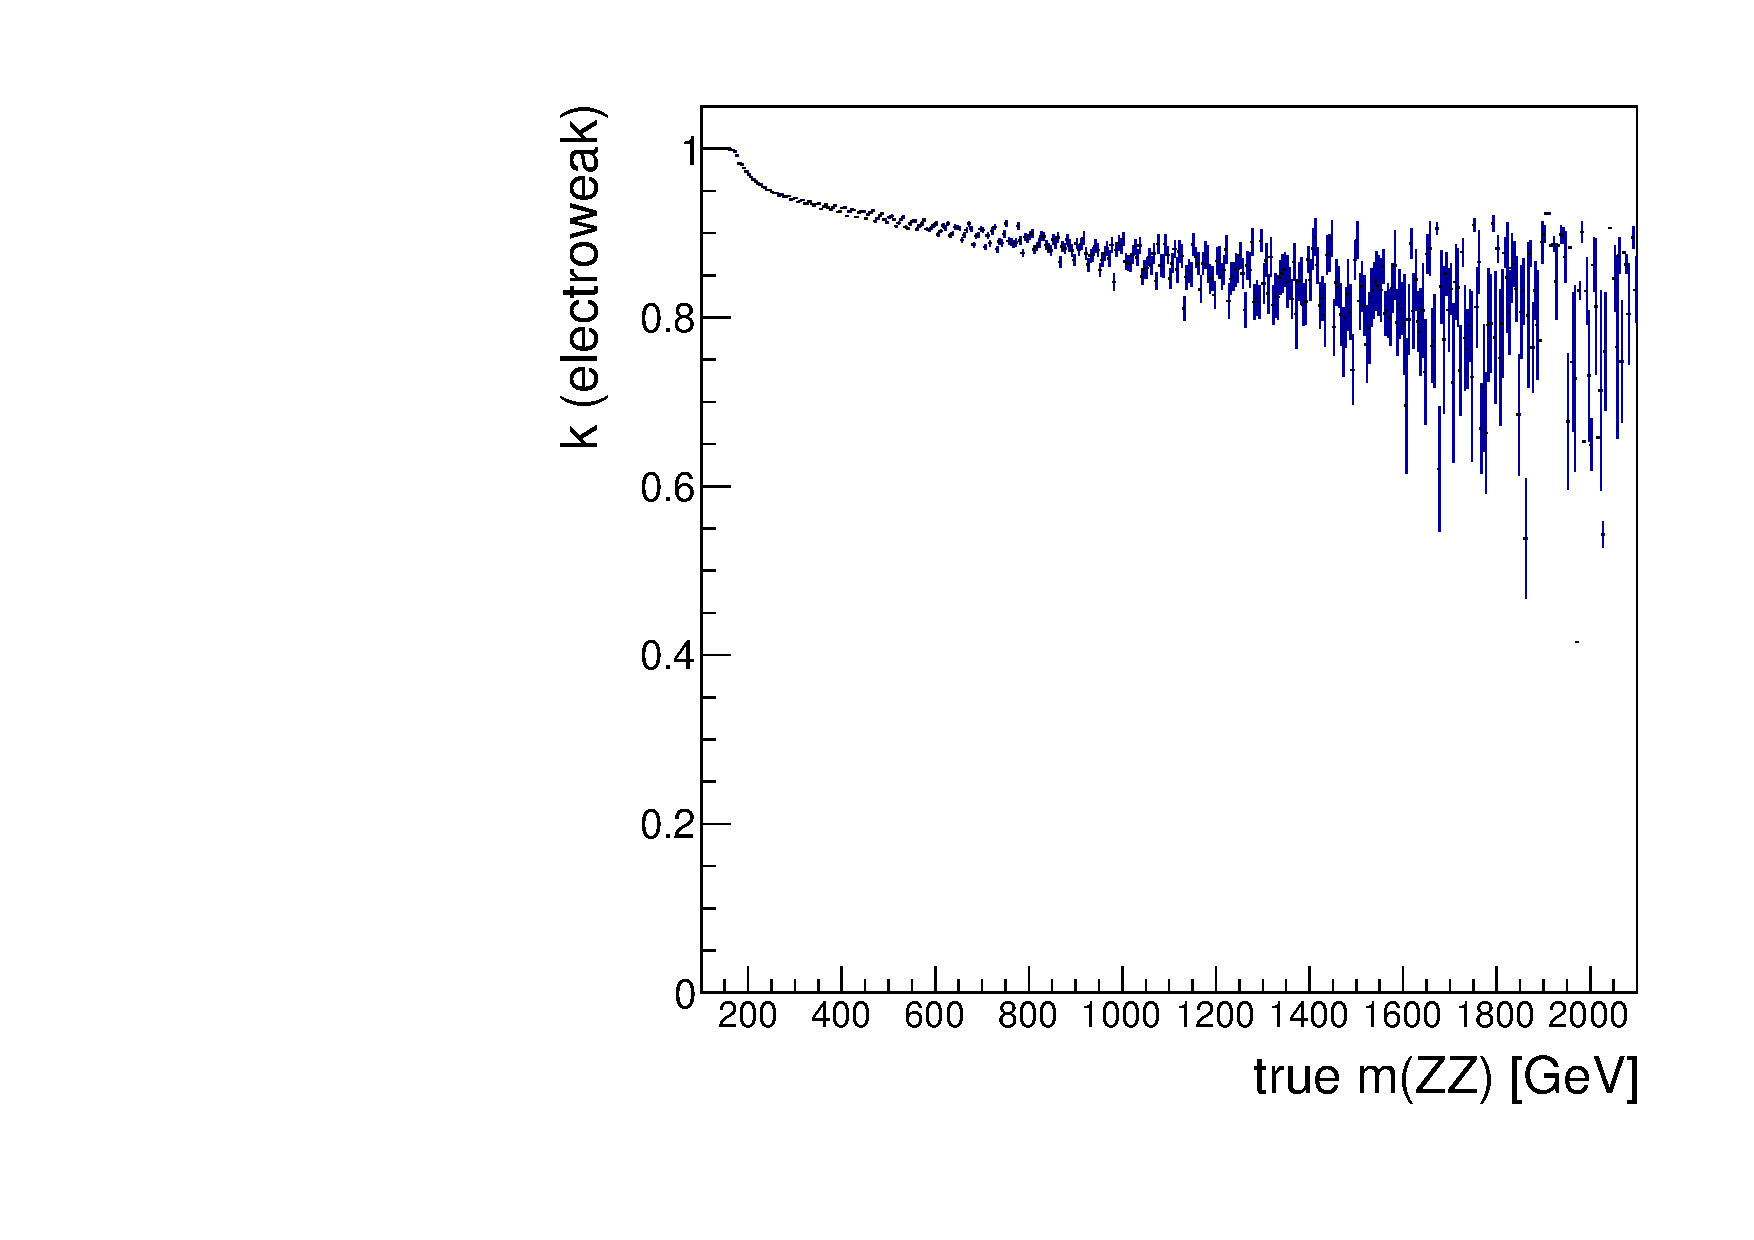
\includegraphics[width=0.48\textwidth]{Figures/IrrBkg/K_ewk_qqZZ.pdf} 
\caption{Left: NNLO/NLO QCD $k$-factor for the \qqZZ~ background as a function of $m(ZZ)$ for the $4\ell$ and $2\ell2\ell^{\prime}$ final states. Right: NLO/NLO electroweak $k$-factor for the \qqZZ~ background as a function of $m(ZZ)$.
\label{fig:qqZZKfactor}}
\end{center}
\end{figure}


\subsection{\ggZZ~ Modelling}

Event simulation for the $\ggZZ$ background is done at LO with the generator \MCFM~7.0~\cite{MCFM,Campbell:2011bn,Campbell:2013una}.
Although no exact calculation exists beyond the LO for the $\ggZZ$ background, 
it has been recently shown~\cite{Bonvini:1304.3053} 
that the soft collinear approximation is able to describe the background cross section and the 
interference term at NNLO\@. Further calculations also show that the K factors are very similar at NLO for the signal 
and background~\cite{Melnikov:2015laa} and at NNLO for the signal and interference terms~\cite{Li:2015jva}. Therefore, the same K factor 
is used for the signal and background~\cite{Passarino:1312.2397v1}. The NNLO K factor for the signal is obtained as a function of $\mllll$ 
using the \textsc{hnnlo}~v2 Monte Carlo program~\cite{Catani:2007vq,Grazzini:2008tf,Grazzini:2013mca} by calculating the NNLO and LO 
$\Pg\Pg\to\PH\to2\ell2\ell^\prime$ cross sections at the small $\PH$ boson decay width of $4.07$~\MeV and taking their ratios. The NNLO as 
well as the NLO K factors and the cross sections from which they are derived are illustrated in Fig.~\ref{fig:ggHZZXsecKfactor}, 
along with the NNLO, NLO and LO cross sections at the SM $\PH$ boson decay width~\cite{Heinemeyer:2013tqa}.
 
\begin{figure}[!htb]
\centering
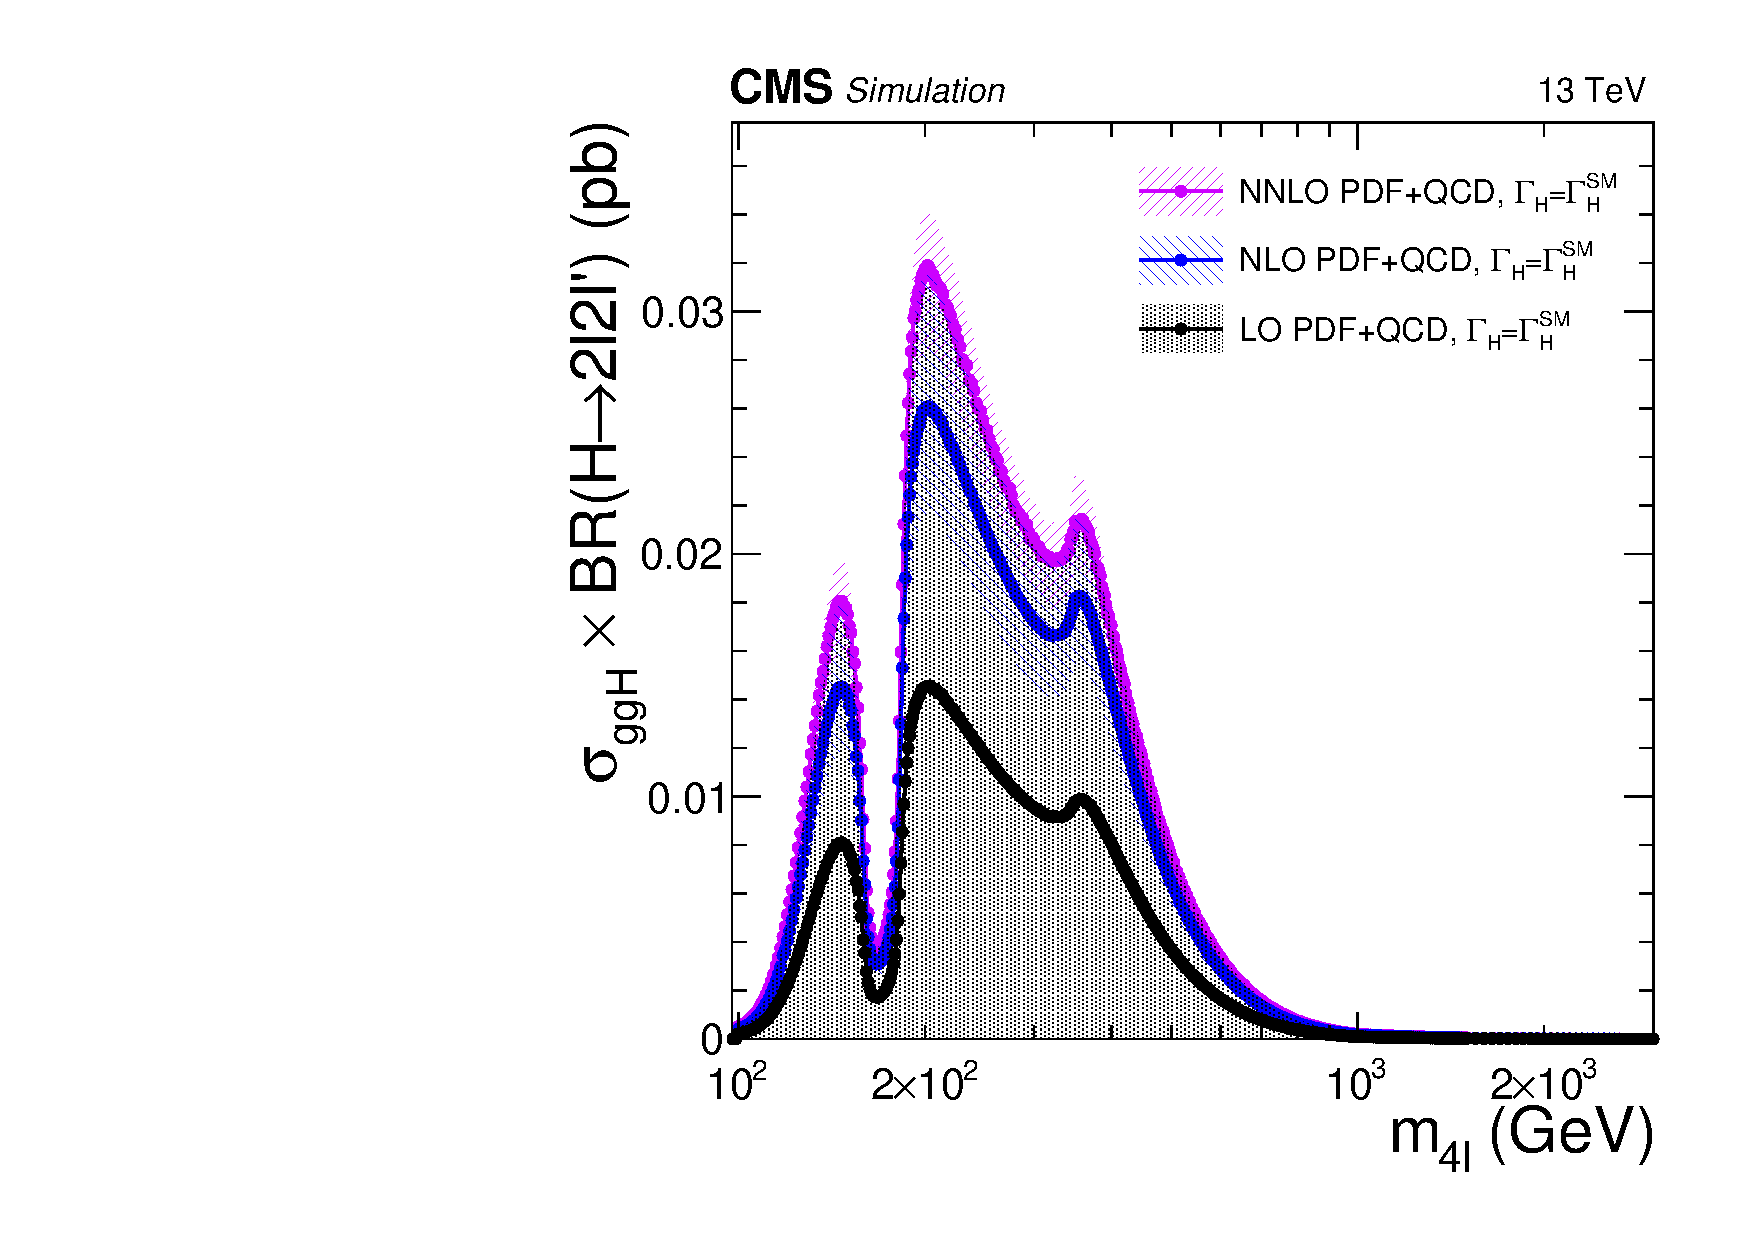
\includegraphics[width=0.48\linewidth]{Figures/IrrBkg/cCompare_hnnlo_ggHZZ2l2l_xsec.pdf}
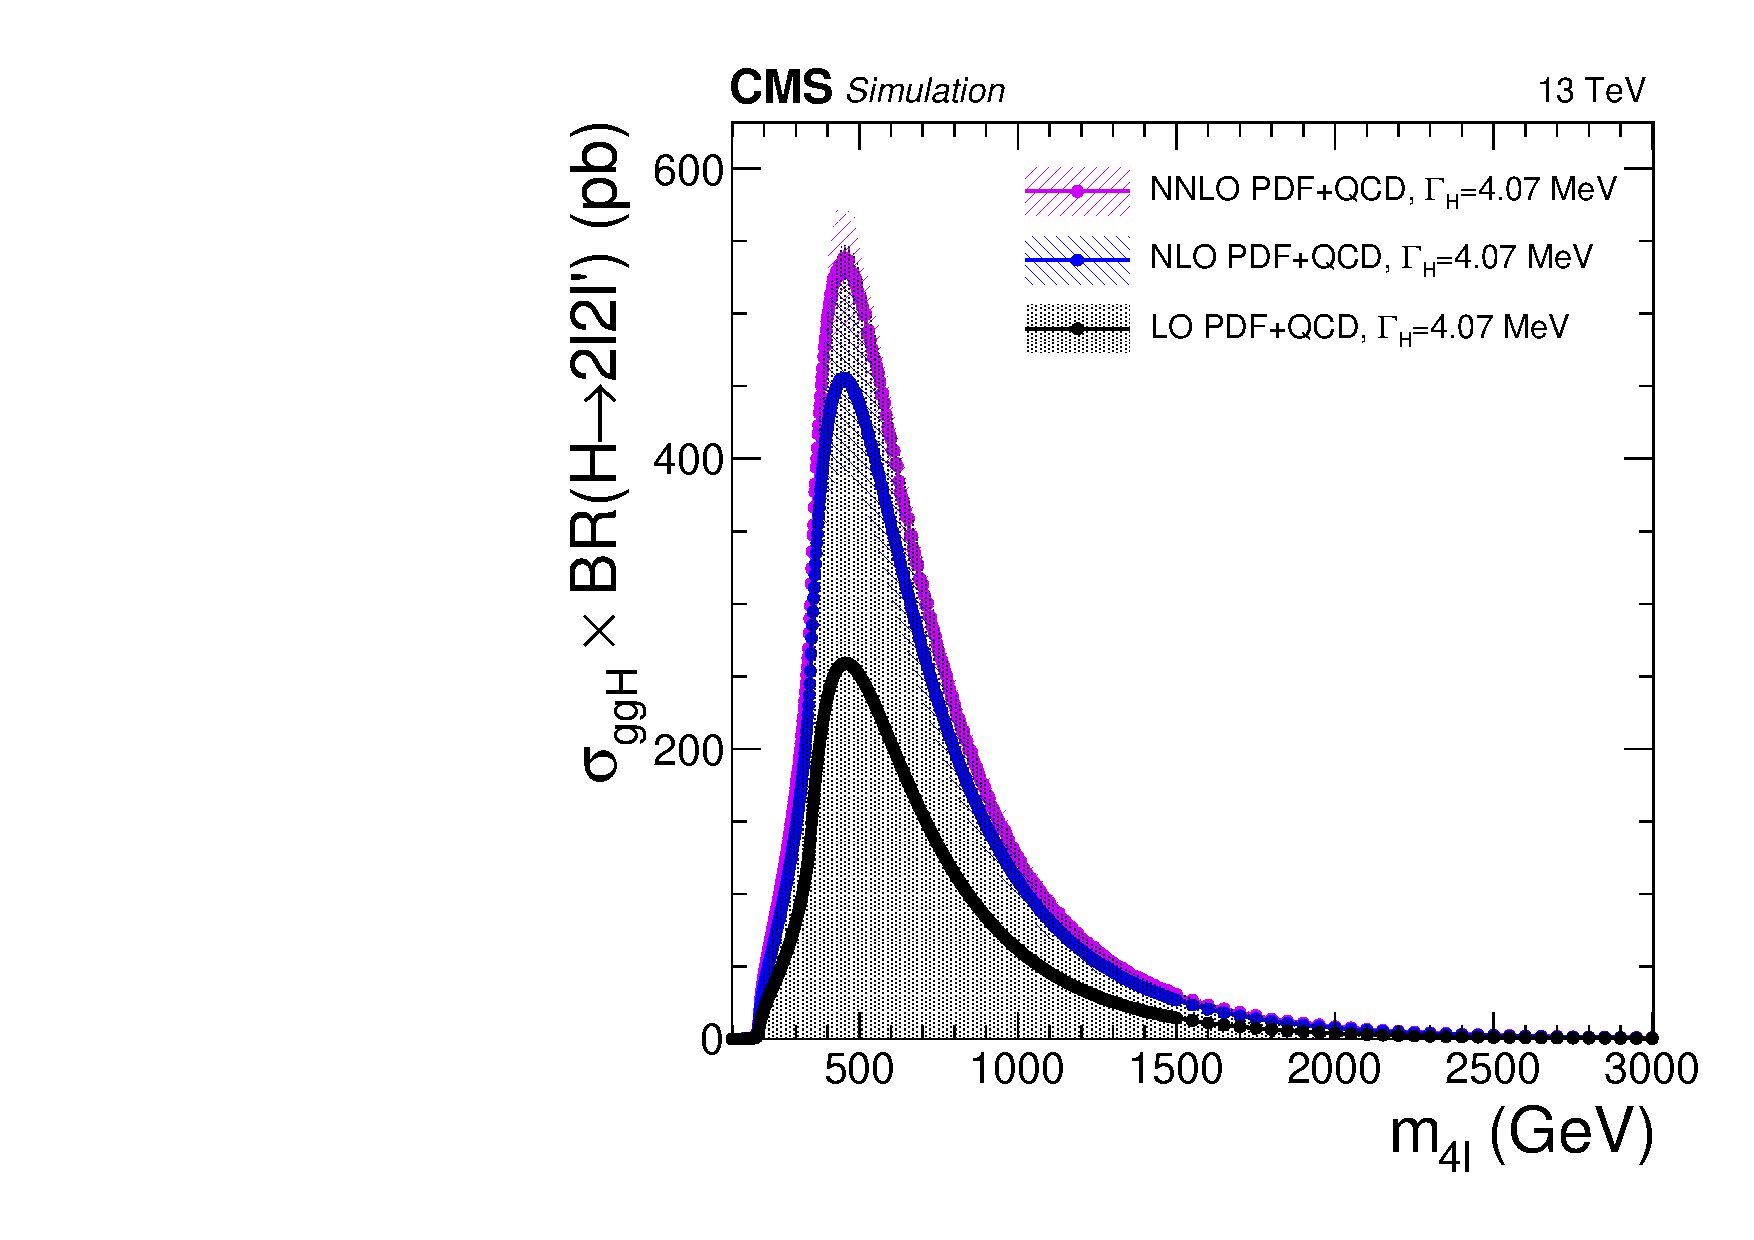
\includegraphics[width=0.48\linewidth]{Figures/IrrBkg/cCompare_hnnlo_ggHZZ2l2l_narrowwidth_xsec.pdf}\\
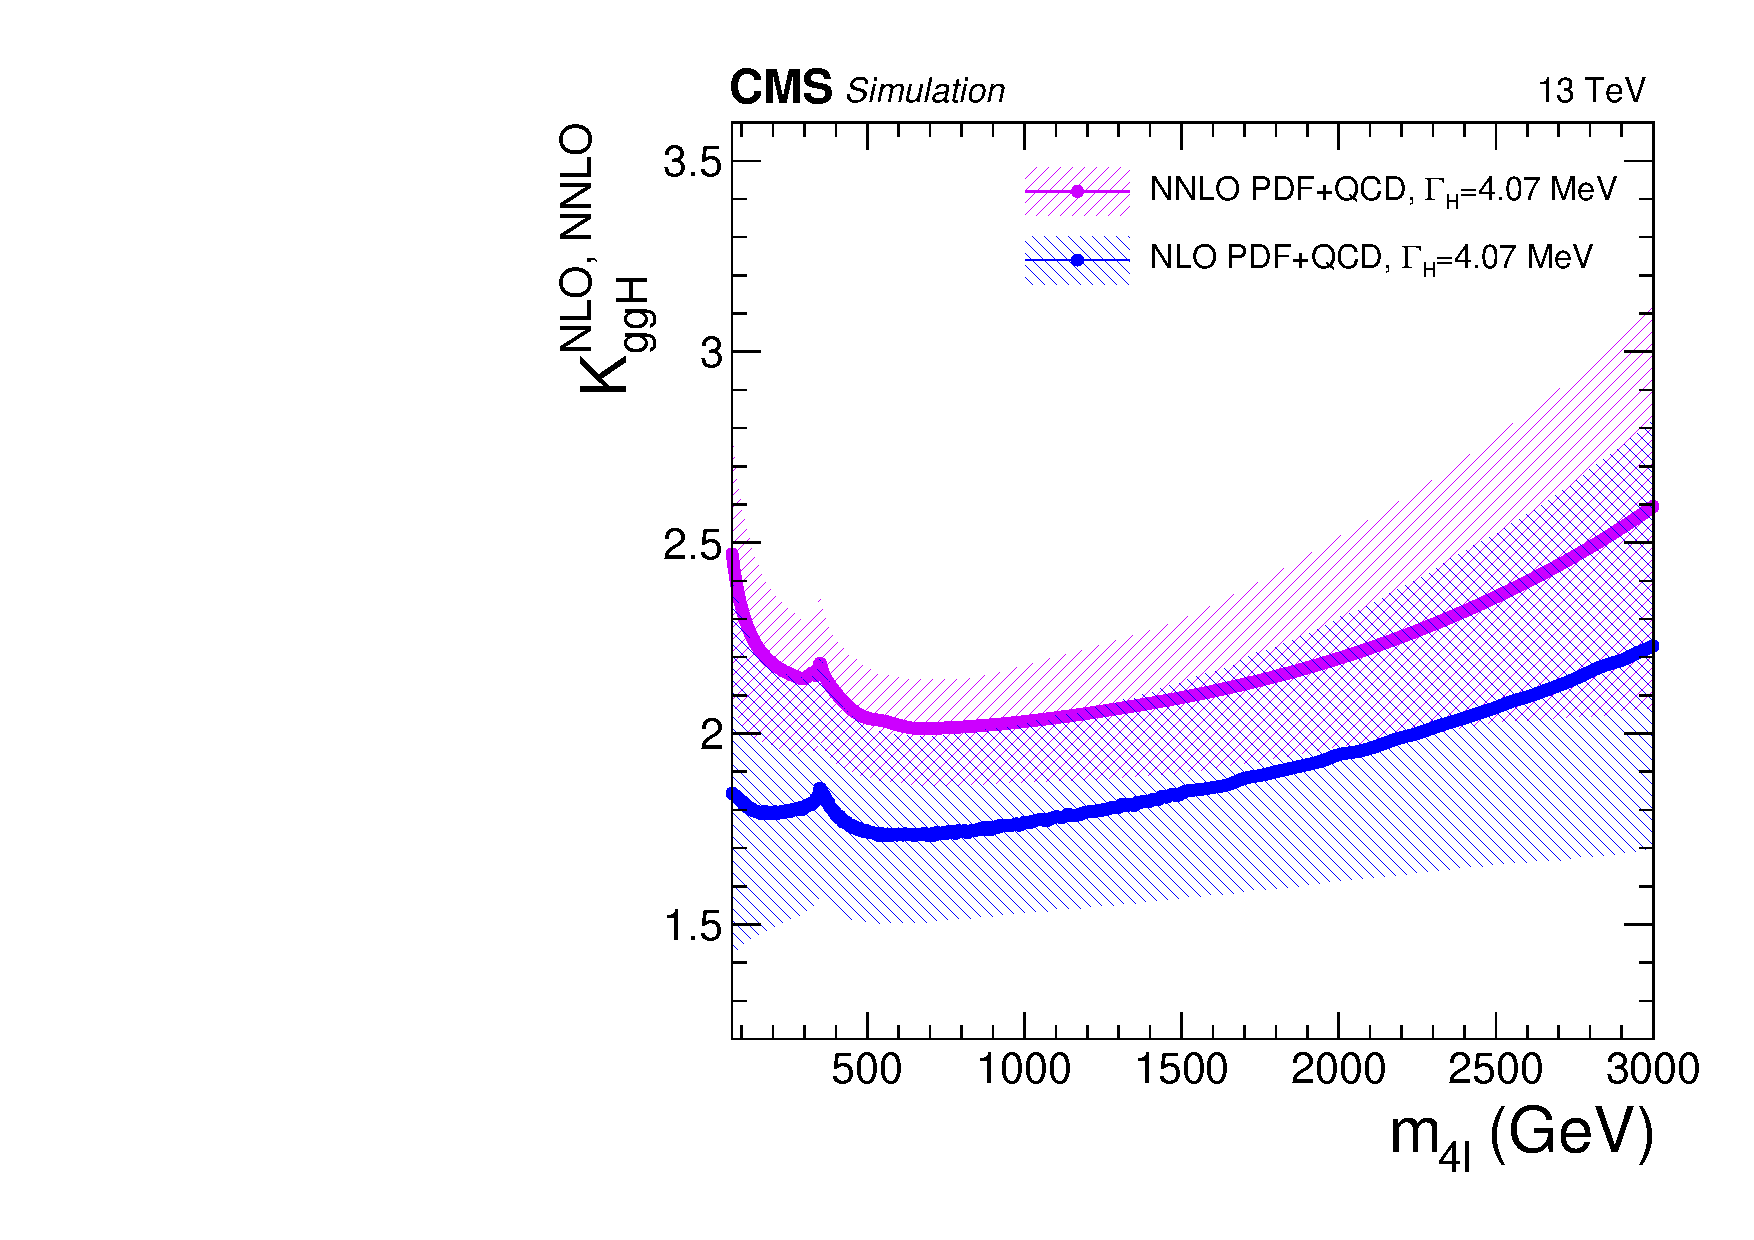
\includegraphics[width=0.48\linewidth]{Figures/IrrBkg/cCompare_hnnlo_ggHZZ2l2l_narrowwidth_kfactor.pdf}
\caption{$\Pg\Pg\to\PH\to2\ell2\ell^\prime$ cross sections at NNLO, NLO and LO at each $\PH$ boson pole mass using the SM $\PH$ boson decay width  (top \cmsLeft) or at the fixed and small decay width of $4.07$~MeV (top \cmsRight). The cross sections using the fixed value are used to obtain the K factor for both the signal and the continuum background contributions as a function of $\mllll$ (bottom).
}
\label{fig:ggHZZXsecKfactor}
\end{figure}


\section{Reducible Background}
\label{sec:zxIntr}
\input{Background/zxIntr.tex}

The reducible background for the $H\to ZZ\to 4\ell $ analysis, hereafter called $Z+X$, originates from processes which contain one or more non-prompt leptons in the four-lepton final state. 
The main sources of non-prompt leptons are non-isolated electrons and muons coming from decays of heavy-flavour mesons, mis-reconstructed jets (usually originating from light-flavour quarks) and electrons from $\gamma$ conversions. 
In this discussion, we will consider a ``fake lepton'' any jet mis-reconstructed as a lepton and any lepton originating from a heavy meson decay.
Similarly, any electron originating from a photon conversion will be considered a ``fake electron''.

In the $H\to ZZ\to 4\ell $ analysis, the rate of these background processes is estimated by measuring the $f_{e}$ and $f_{\mu}$ probabilities for fake electrons and fake muons which do pass the {\bf loose} selection criteria (defined in Section~\ref{sec:eleReco} and~\ref{sec:muonReco}) to also pass the final selection criteria (defined in Section~\ref{sec:zzcandsel}).  
These probabilities, hereafter referred to as fake ratios or fake rates, are applied in dedicated control samples in order to extract the expected background yield in the signal region. 

In the following section, two independent methods are presented to measure both the yields and shapes of the reducible background. The final result combines the outcome of the two approaches. 

\paragraph{Fake Rate Determination (OS Method)}
In order to measure the lepton fake ratios $f_{e}$, $f_{\mu}$, we select samples of $Z(\ell\ell)+e$ and $Z(\ell\ell)+\mu$ events that are expected to be completely dominated by final states which include a $Z$ boson and a fake lepton. 
These events are required to have two same flavour, opposite charge leptons with $p_{T} > 20/10$~GeV passing the tight selection criteria, thus forming the $Z$ candidate. In addition, there is exactly one lepton passing the loose selection criteria as defined above. 
This lepton is used as the probe lepton for the fake ratio measurement. The invariant mass of this lepton and the opposite sign lepton from the reconstructed $Z$ candidate should satisfy $m_{2l} > 4$~GeV. 

% Figure \ref{fig:Z1L_LooseTightVsMZ} shows distributions of the invariant mass of two leptons selected as the ones originating from the Z decay: in case of all loose leptons (top) and in case of loose leptons that pass the tight selection criteria (middle). The distributions for tight leptons show the presence of (asymmetric) conversion of photons that end up with one electron being reconstructed. Figure \ref{fig:Z1L_LooseTightVsMZ} also shows dependance of the electron and muon fake ratios on $M_{inv}(\ell_{1},\ell_{2})$ (bottom). From that it can be concluded that we would benefit by using a tight mass cut on $|M_{inv}(\ell_{1},\ell_{2}) - M_{Z}| < 7$~GeV. By observing the Figure \ref{fig:Z1L_LooseTightVsMET} it can also be concluded that the contamination from $WZ$ and $t \bar{t}$ processes can be greatly suppress by using a $E_{\mathrm{T}}^\text{miss}  < $ 25~GeV.

% %%%%%%%%%%%%%%%%%%%%%%%%
% \begin{figure}[!htb]
% \begin{center}
%    \subfigure [] {\resizebox{7.75cm}{!}{\includegraphics{Figures/RedBkg/mZ1el_EB_d_process_auto.pdf}}} 
%    \subfigure [] {\resizebox{7.75cm}{!}{\includegraphics{Figures/RedBkg/mZ1mu_EB_d_process_auto.pdf}}} \\
%    \subfigure [] {\resizebox{7.75cm}{!}{\includegraphics{Figures/RedBkg/mZ1el_EB_n_process_auto.pdf}}} 
%    \subfigure [] {\resizebox{7.75cm}{!}{\includegraphics{Figures/RedBkg/mZ1mu_EB_n_process_auto.pdf}}} \\
%   \caption{
% Distribution of the invariant mass of two leptons selected as the ones originating form the Z decay. Distributions are shown for the $Z(\ell\ell)+e$ (left) and $Z(\ell\ell)+\mu$ (right) samples, as defined in the text. The top row corresponds to all the events where we have the additional lepton passing the loose criteria, while middle row shows distributions for events when the loose lepton passes the tight selection criteria. }
% \label{fig:Z1L_LooseTightVsMZ}
% \end{center}
% \end{figure}
% %%%%%%%%%%%%%%%%%%%%%%%
% \begin{figure}[!htb]
% \begin{center}
%  \subfigure [] {\resizebox{7.75cm}{!}{\includegraphics{Figures/RedBkg/FR_electrons_mZ1_Data.pdf}}} 
%  \subfigure [] {\resizebox{7.75cm}{!}{\includegraphics{Figures/RedBkg/FR_muons_mZ1_Data.pdf}}} 
% \caption{
% Fake Rate at which electrons (muons), that pass the loose criteria, also pass the tight criteria. Distributions of $|M_{inv}(\ell_{1},\ell_{2})|$ show dependence of the fake ratios in the region below 85~GeV.
% }
% \label{fig:Z1L_LooseTightVsMZFR}
% \end{center}
% \end{figure}
% %%%%%%%%%%%%%%%%%%%%%%%
% \begin{figure}[!htb]
% \begin{center}
%    \subfigure [] {\resizebox{7.75cm}{!}{\includegraphics{Figures/RedBkg/mEtel_EB_d_process_auto.pdf}}} 
%    \subfigure [] {\resizebox{7.75cm}{!}{\includegraphics{Figures/RedBkg/mEtmu_EB_d_process_auto.pdf}}} \\
%    \subfigure [] {\resizebox{7.75cm}{!}{\includegraphics{Figures/RedBkg/mEtel_EB_n_process_auto.pdf}}} 
%    \subfigure [] {\resizebox{7.75cm}{!}{\includegraphics{Figures/RedBkg/mEtmu_EB_n_process_auto.pdf}}}
% \caption{
% Distribution of the of $E_{\mathrm{T}}^\text{miss}  $. Distributions are shown for the $Z(\ell\ell)+e$ (left) and $Z(\ell\ell)+\mu$ (right) samples, as defined in the text. The top row corresponds to all the events where we have the additional lepton passing the loose criteria, while bottom row shows distributions for events when the loose lepton passes the tight selection criteria.
% }
% \label{fig:Z1L_LooseTightVsMET}
% \end{center}
% \end{figure}
% %%%%%%%%%%%%%%%%%%%%%%%

The fake ratios are evaluated using the tight requirement 
$|M_{inv}(\ell_{1},\ell_{2}) - M_{Z}| < 7 $~GeV, to reduce the 
contribution from photon (asymmetric) conversions populating low masses. 
The fake ratios are measured in bins of the transverse momentum of the loose lepton and barrel and endcap region.

The electron and muon fake rates are measured within 
$|M_{inv}(\ell_{1},\ell_{2}) - M_{Z}| < 7 $~GeV and $E_{\mathrm{T}}^\text{miss}  < $ 25~GeV are 
shown in Figure~\ref{fig:os_fakerates}. 

\begin{figure}[!htb]
\begin{center}
    \subfigure [] {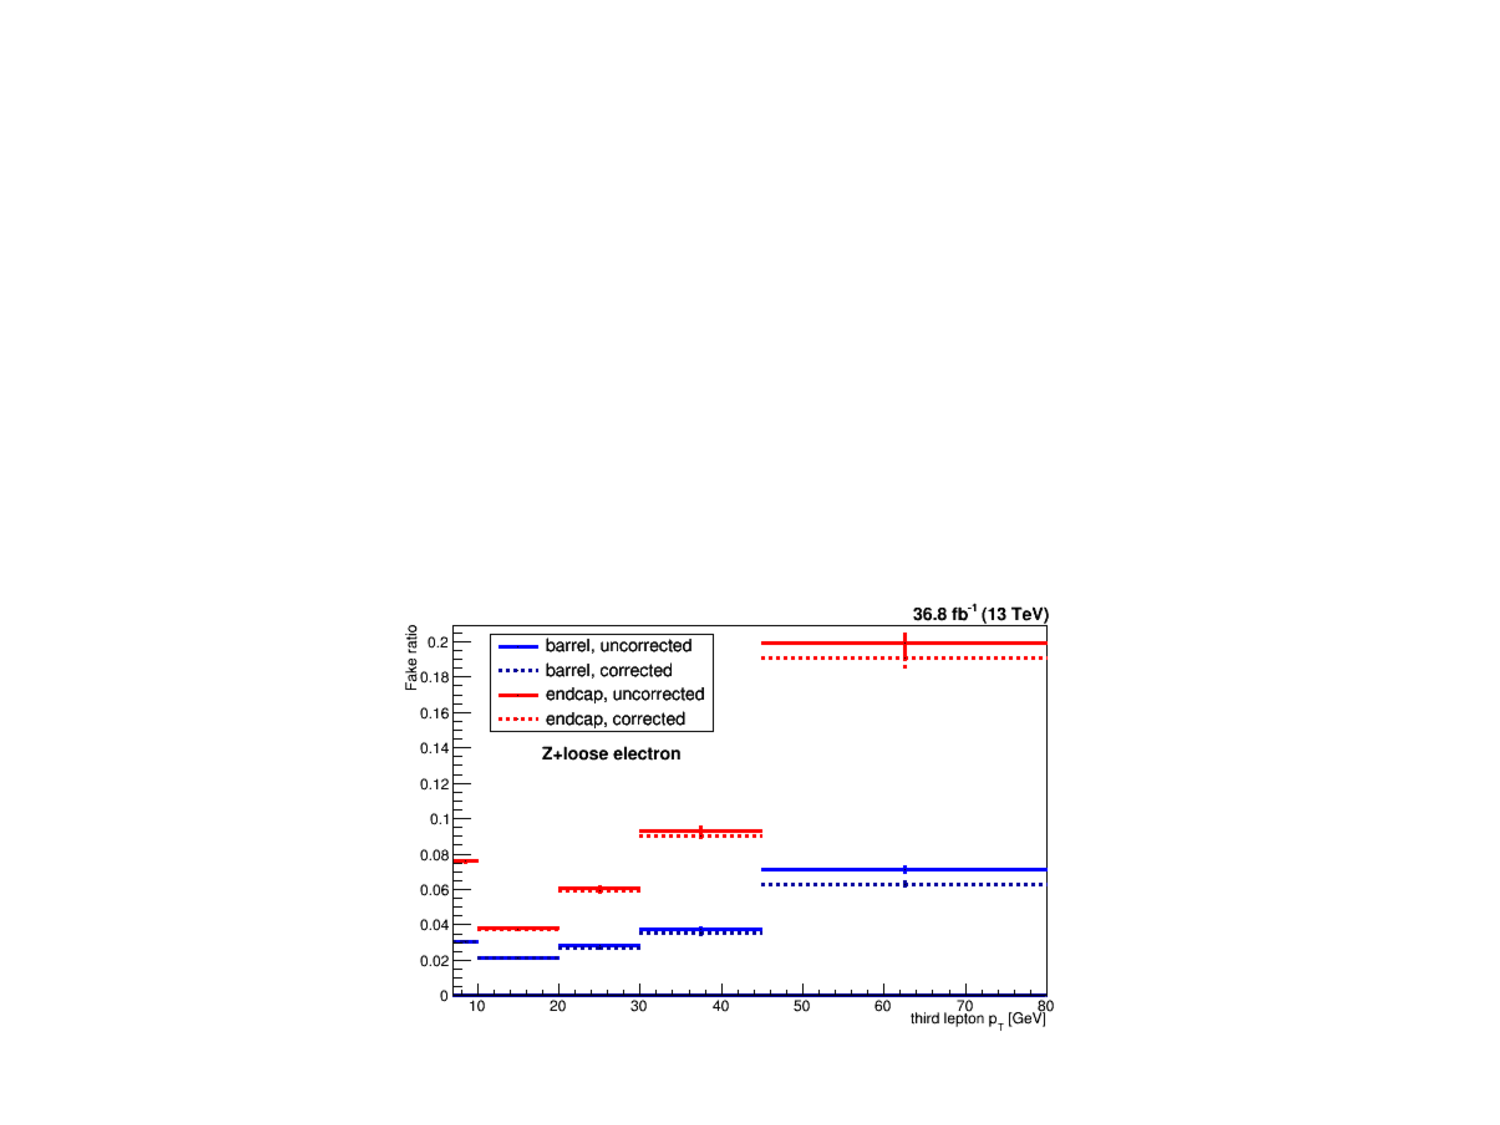
\includegraphics [width=0.45\textwidth]{Figures/RedBkg/FR_electrons_ptl3_DataallTR.pdf}}
    \subfigure [] {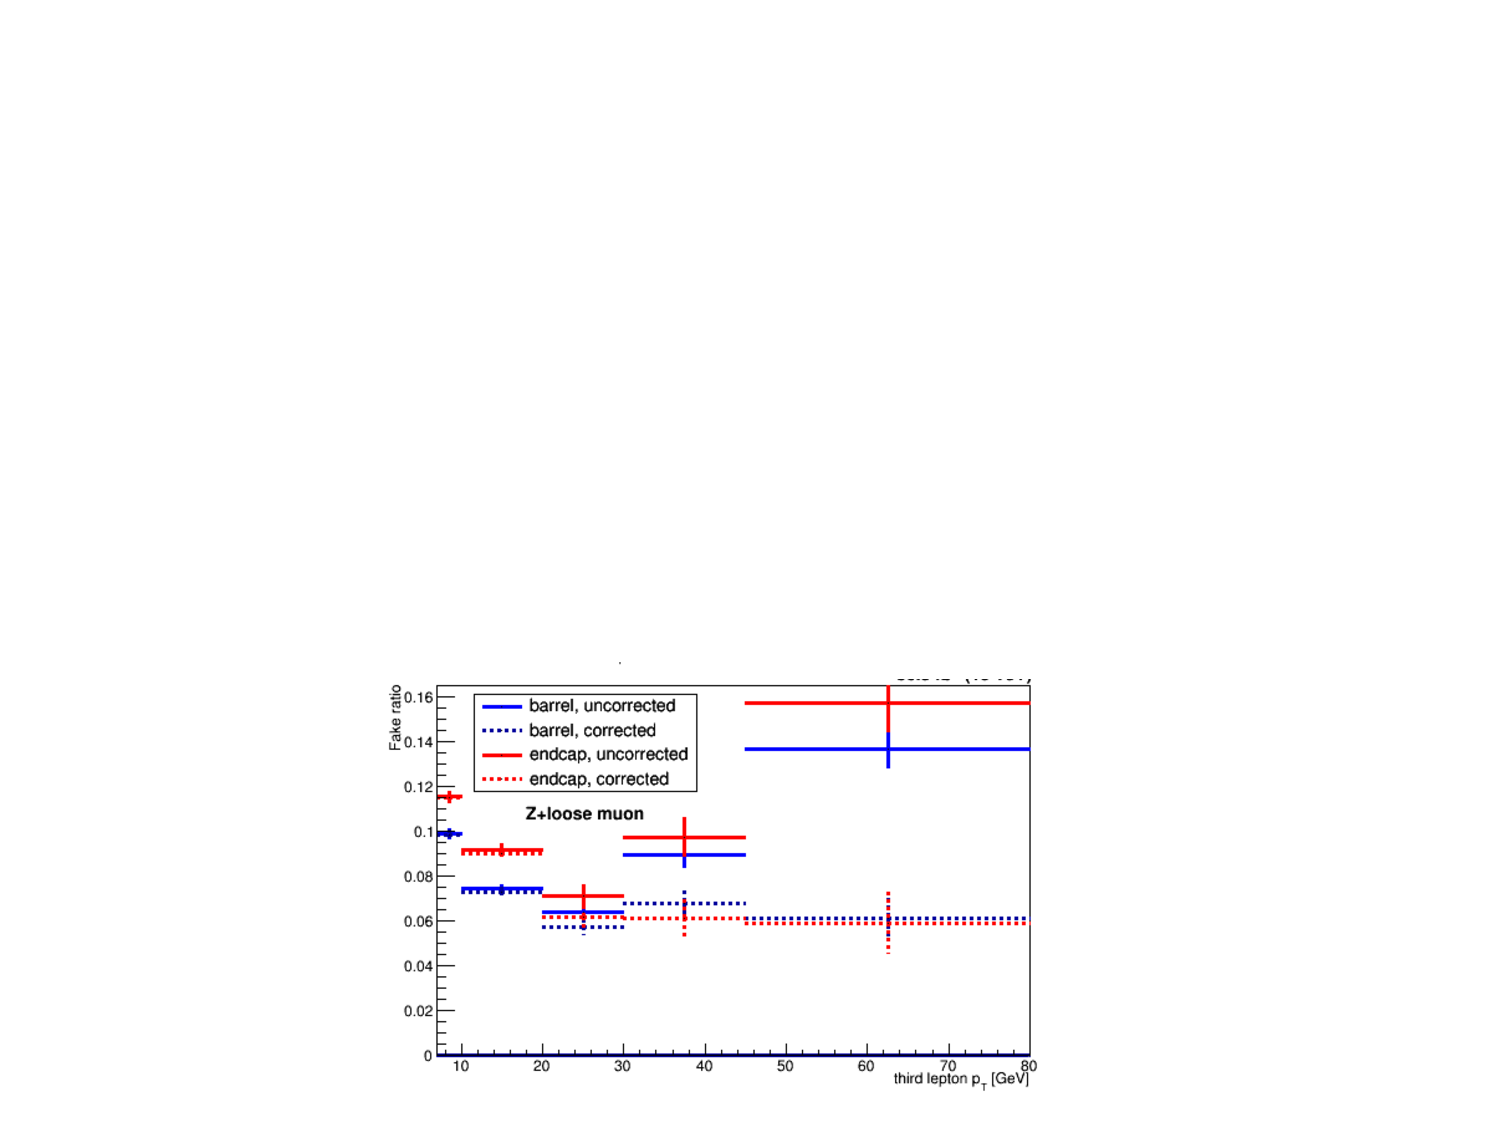
\includegraphics [width=0.45\textwidth]{Figures/RedBkg/FR_muons_ptl3_DataallTR.pdf}}
  \caption{
Fake rates as a function of the probe $p_T$ for  electrons (a) and muons (b) which satisfy the loose selection criteria, measured in
a $Z(\ell\ell)+\ell$ sample in the $13$~TeV data.
The barrel selection includes electrons (muons) up to $|\eta|$ = 1.479 (1.2).
}
\label{fig:os_fakerates}
\end{center}
\end{figure}



\paragraph{Fake Rate Application (OS Method)}
\label{sec:zxA}

Two control samples are obtained as subsets of four lepton events
which pass the first step of the selection ({\it First Z} step, see
section~\ref{sec:zzcandsel}), requiring an additional pair of 
loose leptons of same flavour 
and opposite charge, that pass the ${\rm SIP_{3D}}$ cut. 
The events must satisfy all kinematic cuts applied for the {\it Higgs phase space} selection
(see~\ref{sec:zzcandsel}).
The first control sample is obtained by
requiring that the two loose leptons which do not make the $Z_1$ candidate 
do not pass the final identification and
isolation criteria.
The other two leptons pass
the final selection criteria by definition of the $Z_1$. 
This sample is denoted as ``2 Prompt + 2
Fail'' ({\it 2P+2F}) sample. It is expected to be populated with
events that intrinsically have only two prompt leptons 
(mostly $DY$, with a small fraction of $t \bar{t}$ and $Z \gamma$ events).
The second control sample is obtained by requiring one of
the four leptons not to pass the final identification and isolation
criteria.
The other three
leptons should pass the final selection criteria. This control sample
is denoted as ``3 Prompt + 1 Fail'' ({\it 3P+1F}) sample. It is
expected to be populated with the type of events that populate the
2P+2F region, 
albeit with different relative proportions,
as well as with $WZ$ events that intrinsically have three
prompt leptons.


The control samples obtained in this way, orthogonal by construction
to the signal region, are enriched with fake leptons and are used to
estimate the reducible background in the signal
region. 

The invariant mass distribution of events selected in the 2P+2F control sample
is shown in Fig.~\ref{fig:2P2F_dataMC} for the $13$~TeV dataset. 

\begin{figure}[!htb]
\begin{center}
    {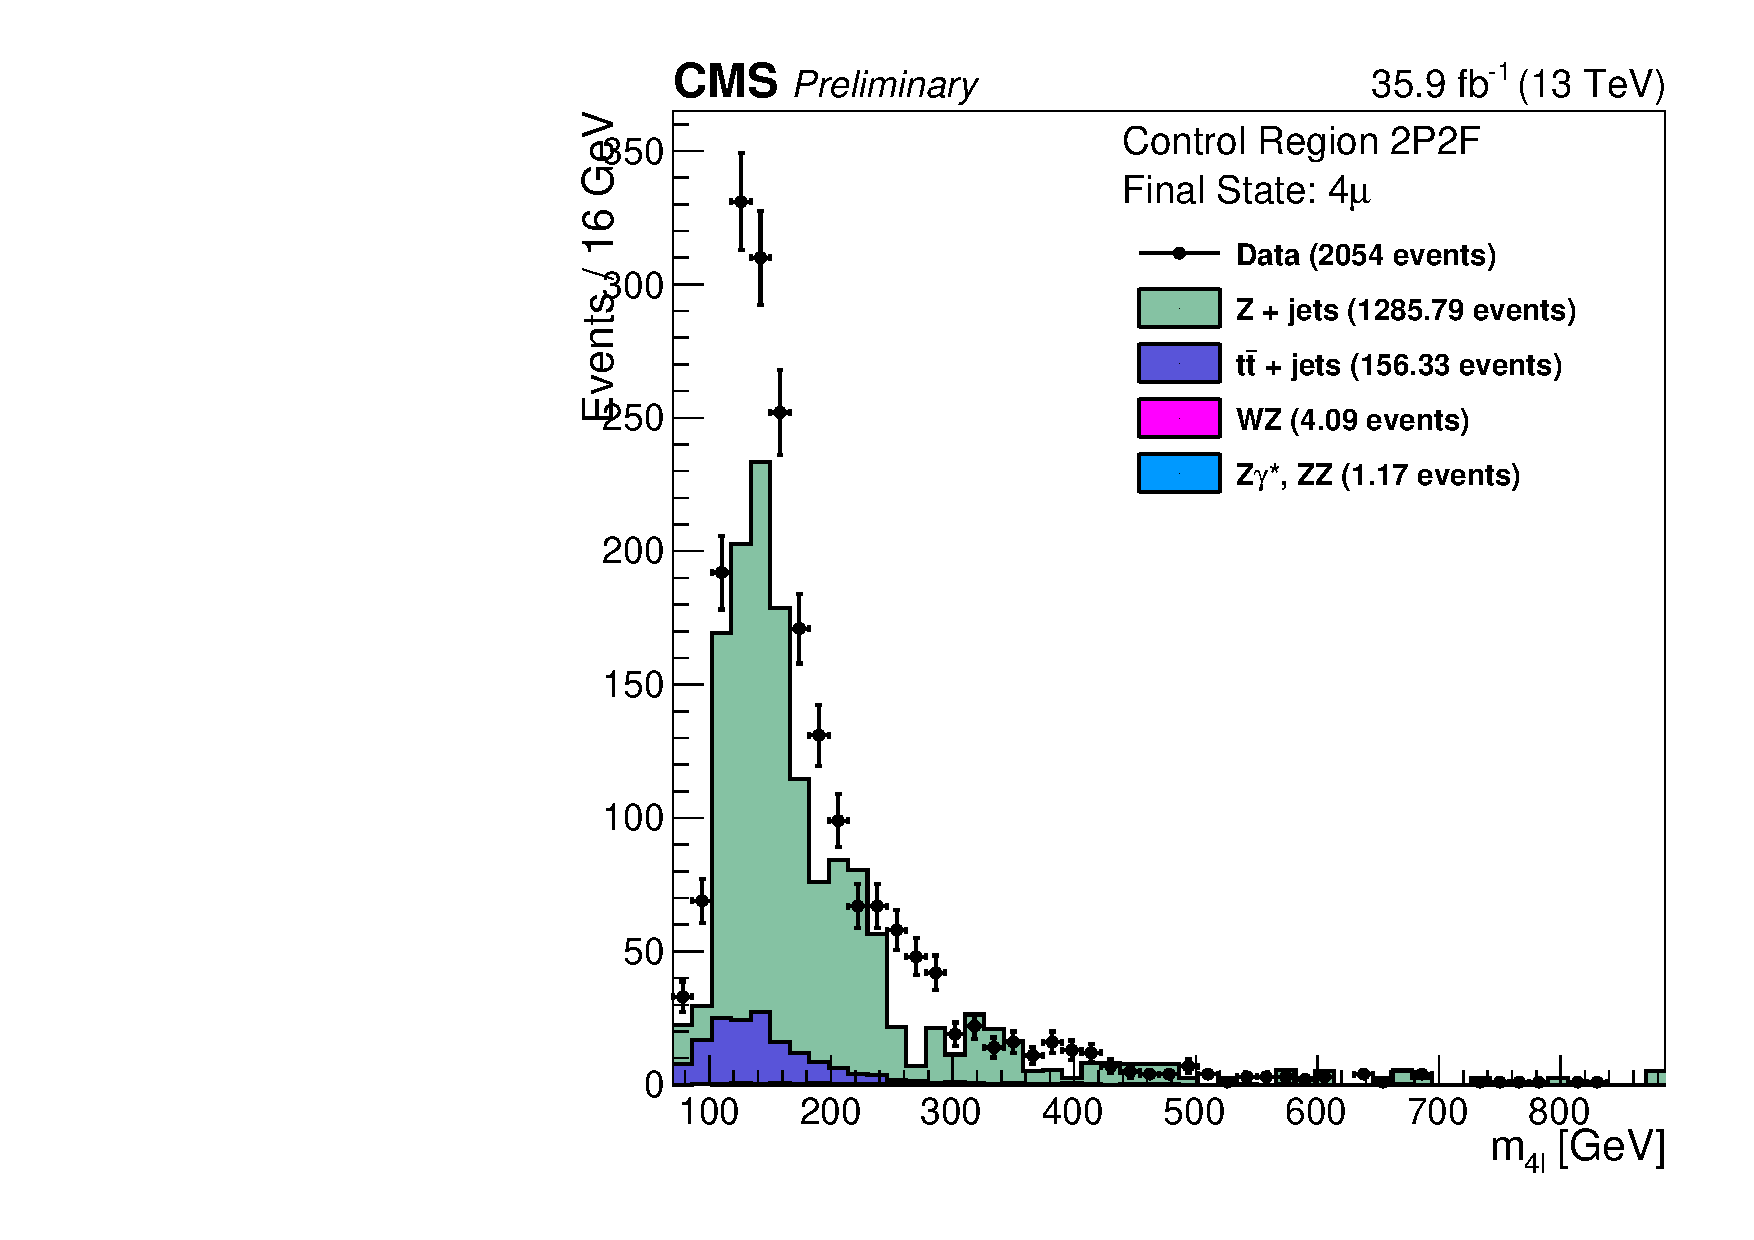
\includegraphics [width=0.45\textwidth] {Figures/RedBkg/HZZ_2P2Fuw_ZZMass_4m.pdf}}
    {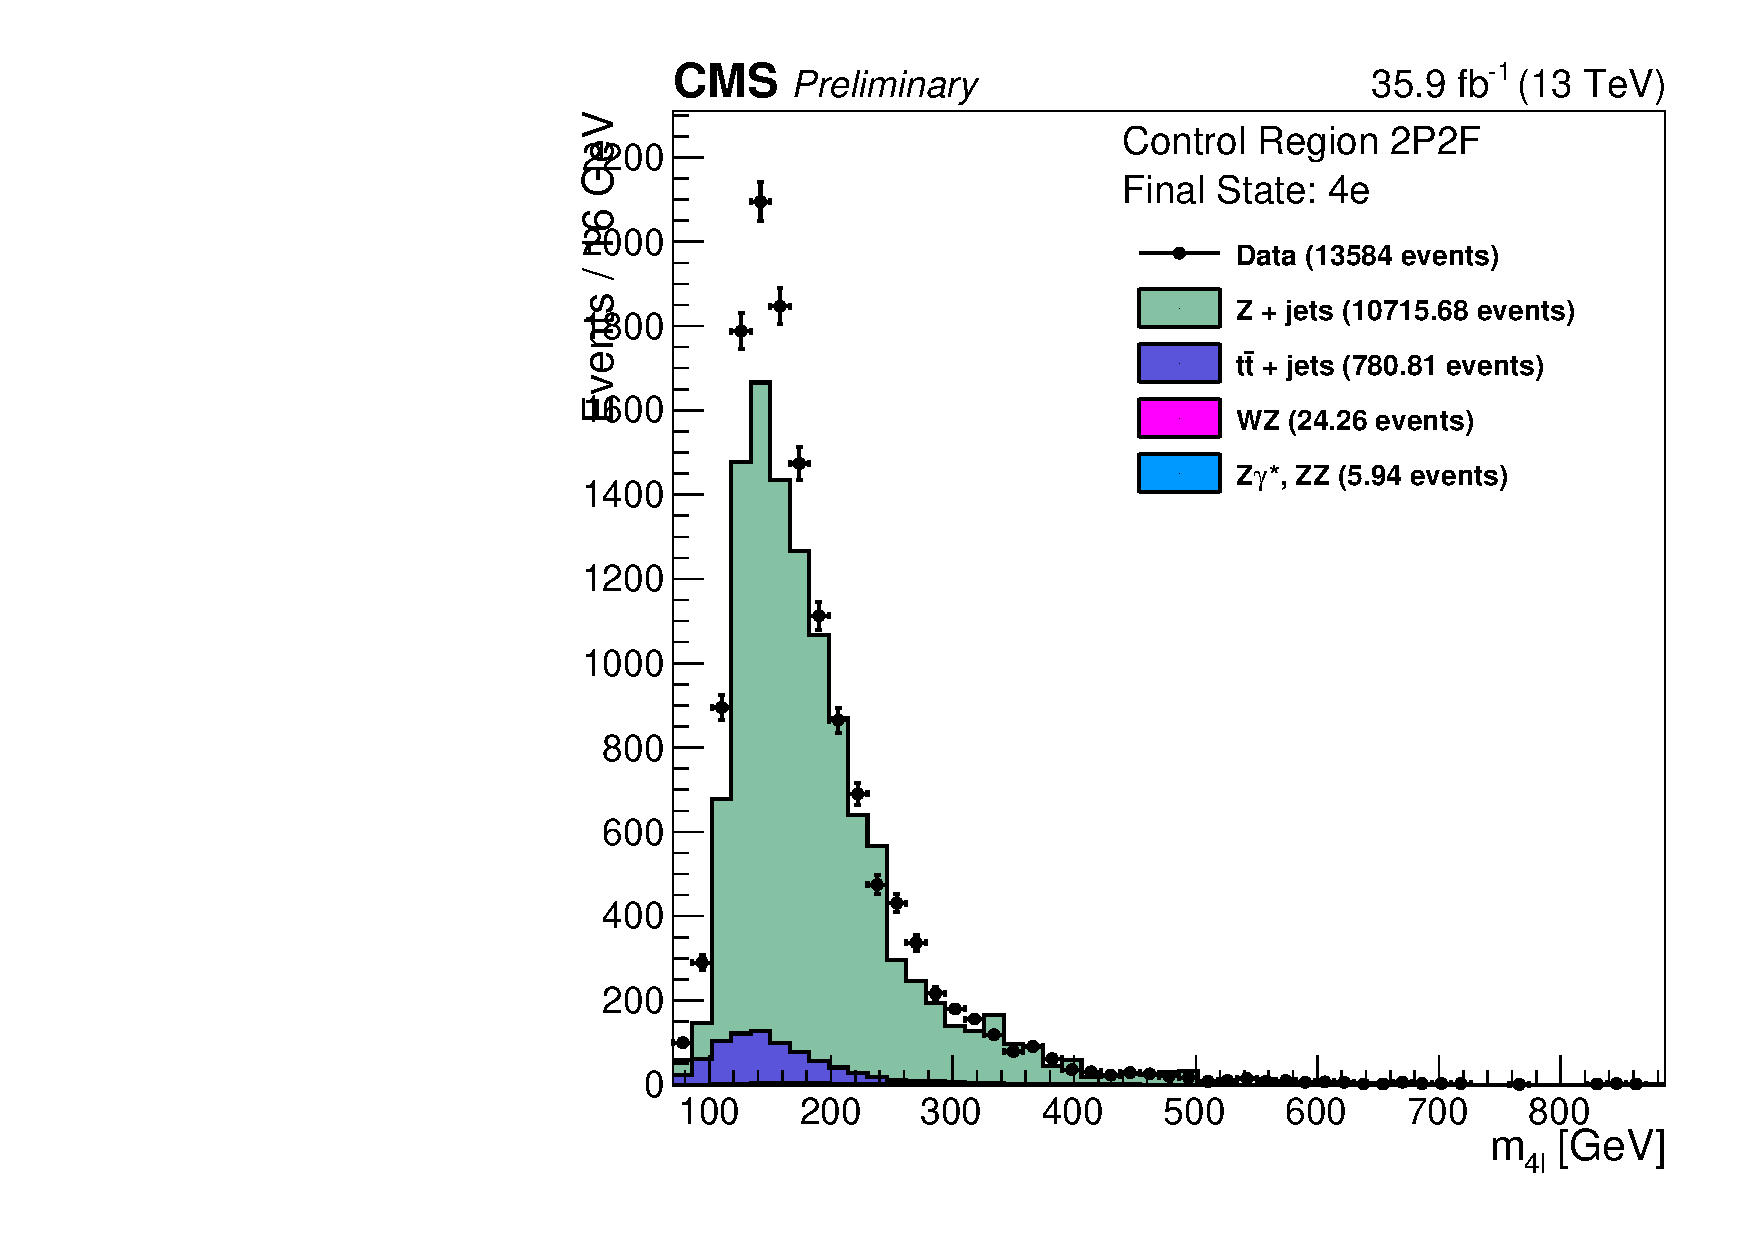
\includegraphics [width=0.45\textwidth] {Figures/RedBkg/HZZ_2P2Fuw_ZZMass_4e.pdf}} \\
    {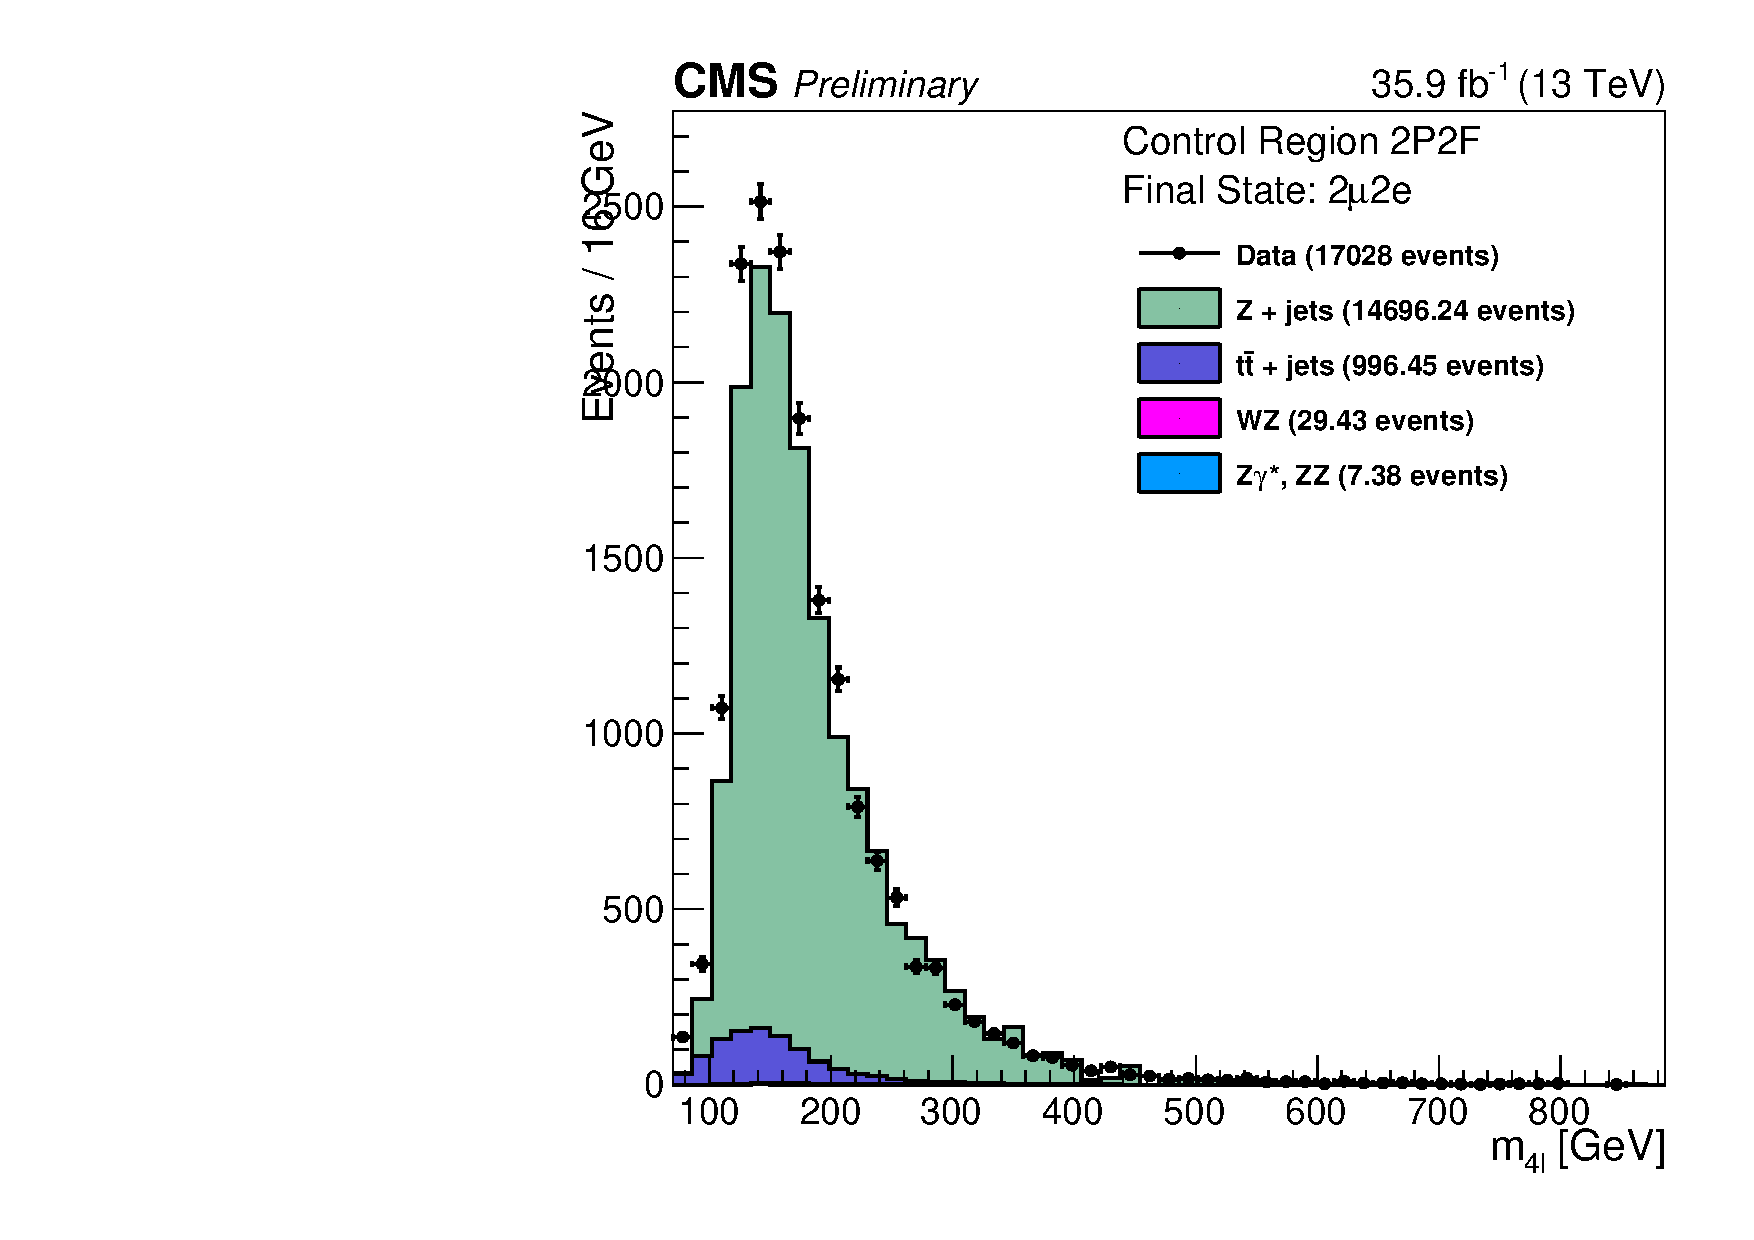
\includegraphics [width=0.45\textwidth] {Figures/RedBkg/HZZ_2P2Fuw_ZZMass_2m2e.pdf}}
    {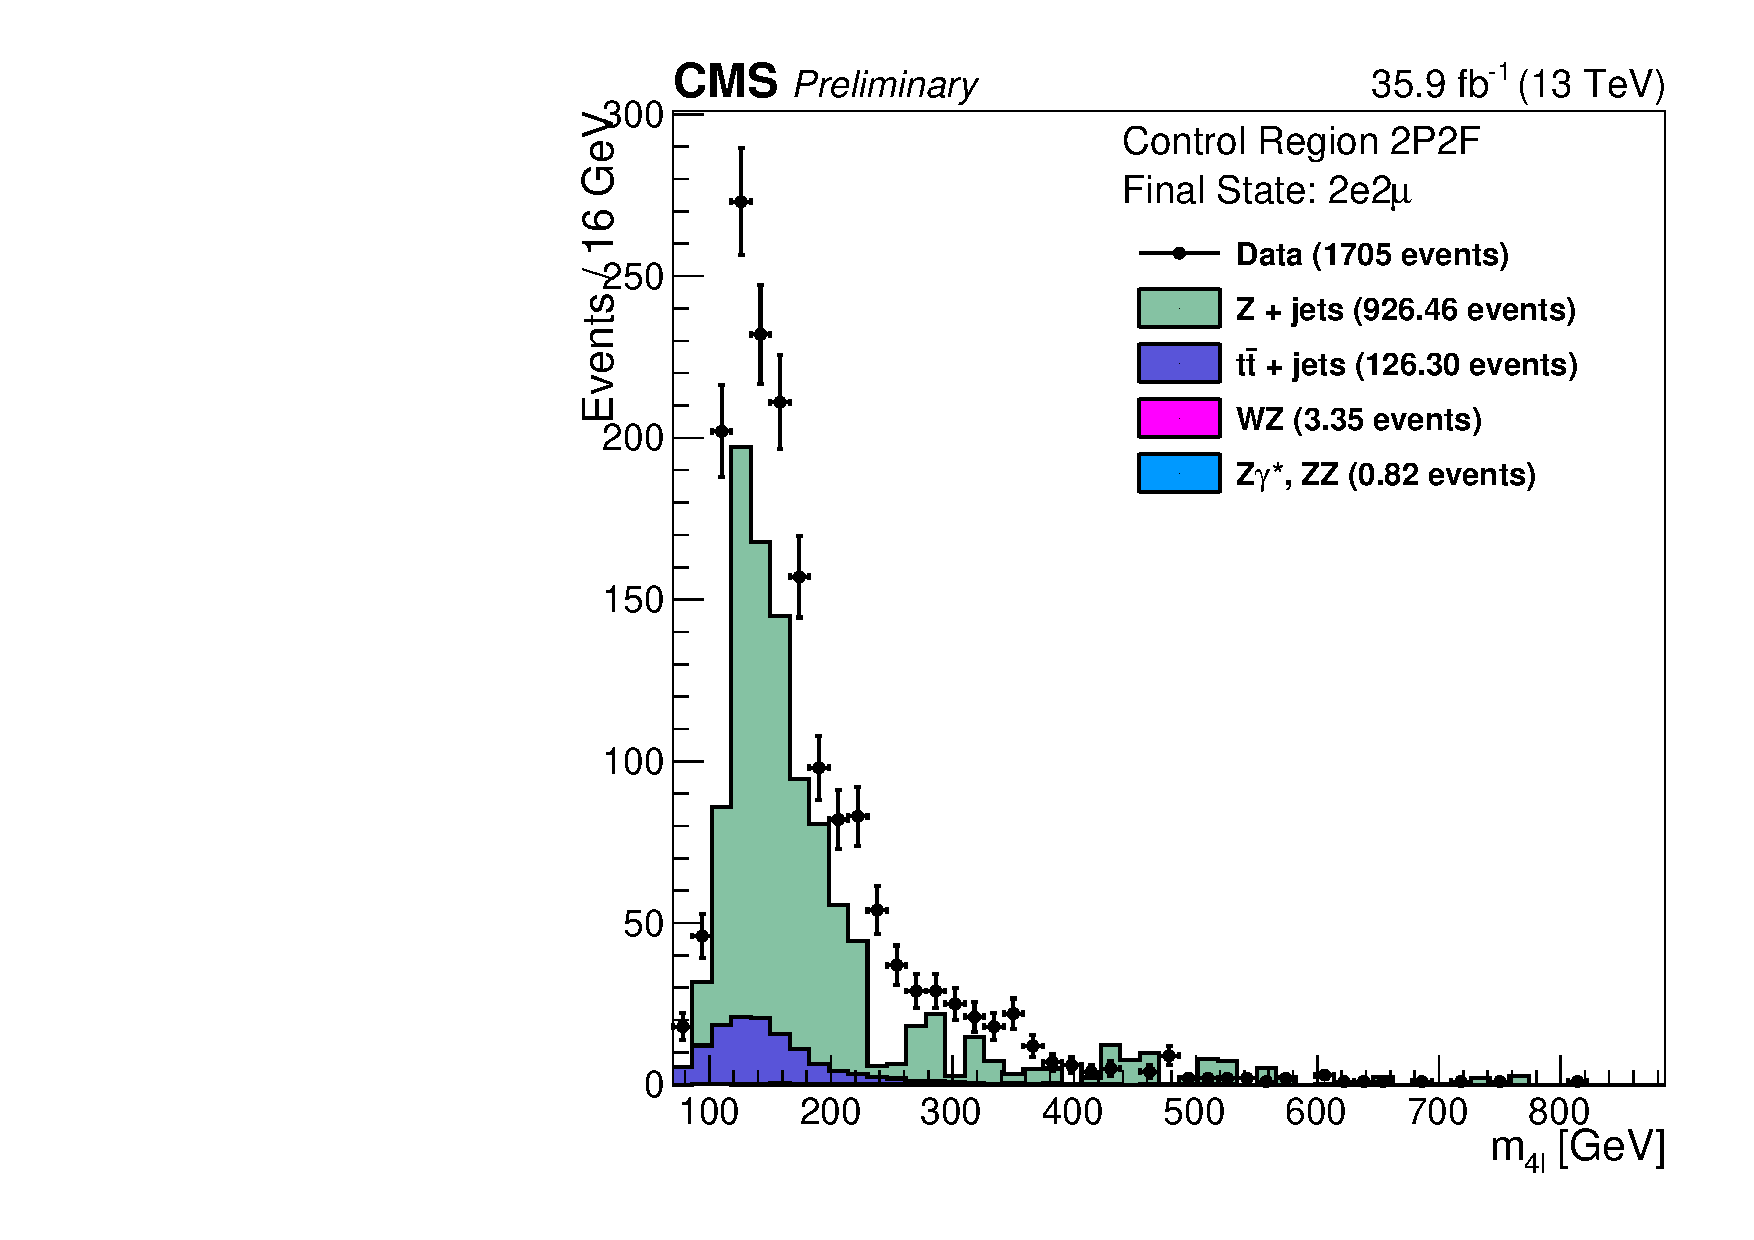
\includegraphics [width=0.45\textwidth] {Figures/RedBkg/HZZ_2P2Fuw_ZZMass_2e2m.pdf}} \\
\caption{
Invariant mass distribution of the events selected in the 2P+2F control sample in the
$13$~TeV dataset, (top left)  $4\mu$ , (top right) $4e$ , (bottom left)  $2\mu2e$ and (bottom right)  $2e2\mu$ channels.
}
\label{fig:2P2F_dataMC}
\end{center}
\end{figure}

\begin{figure}[!htb]
\begin{center}
    {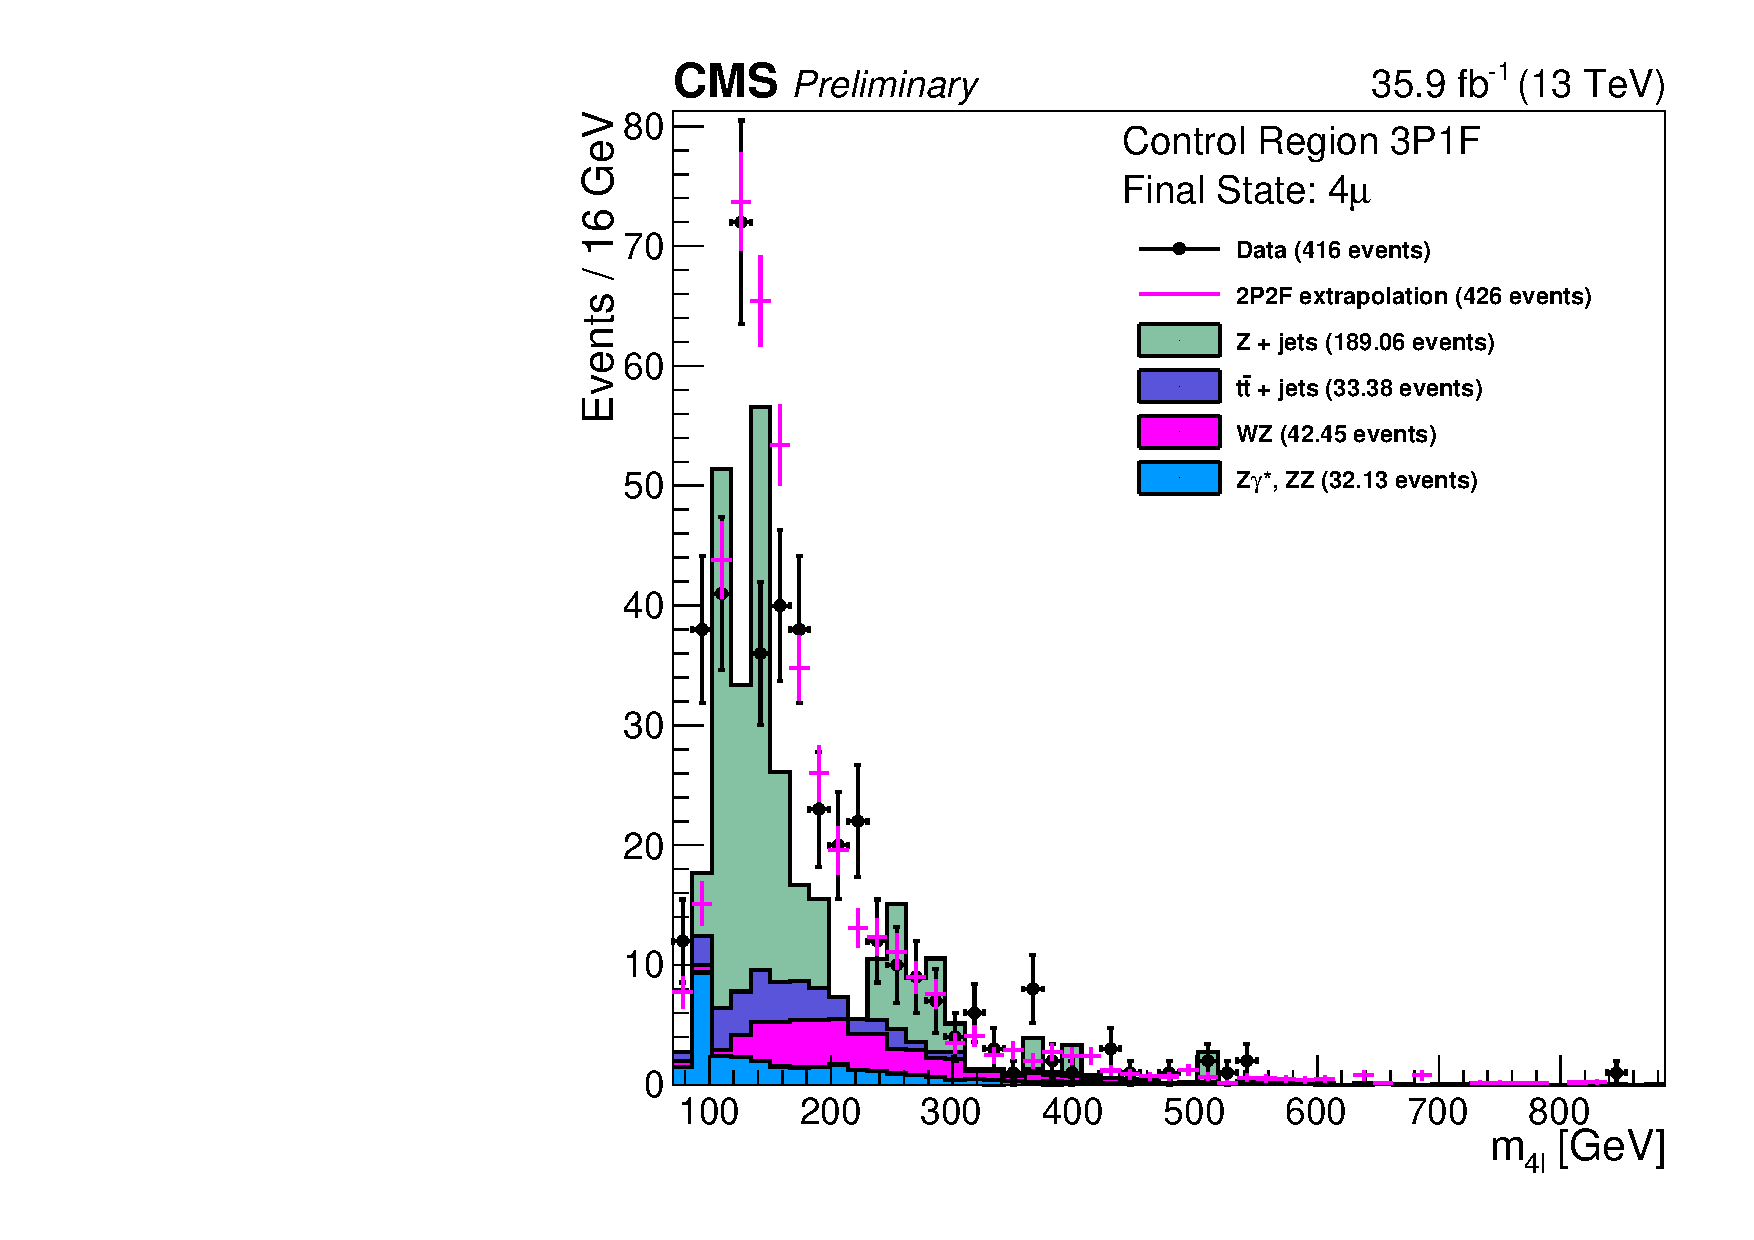
\includegraphics [width=0.45\textwidth] {Figures/RedBkg/HZZ_3P1Fuw_ZZMass_4m.pdf}}
    {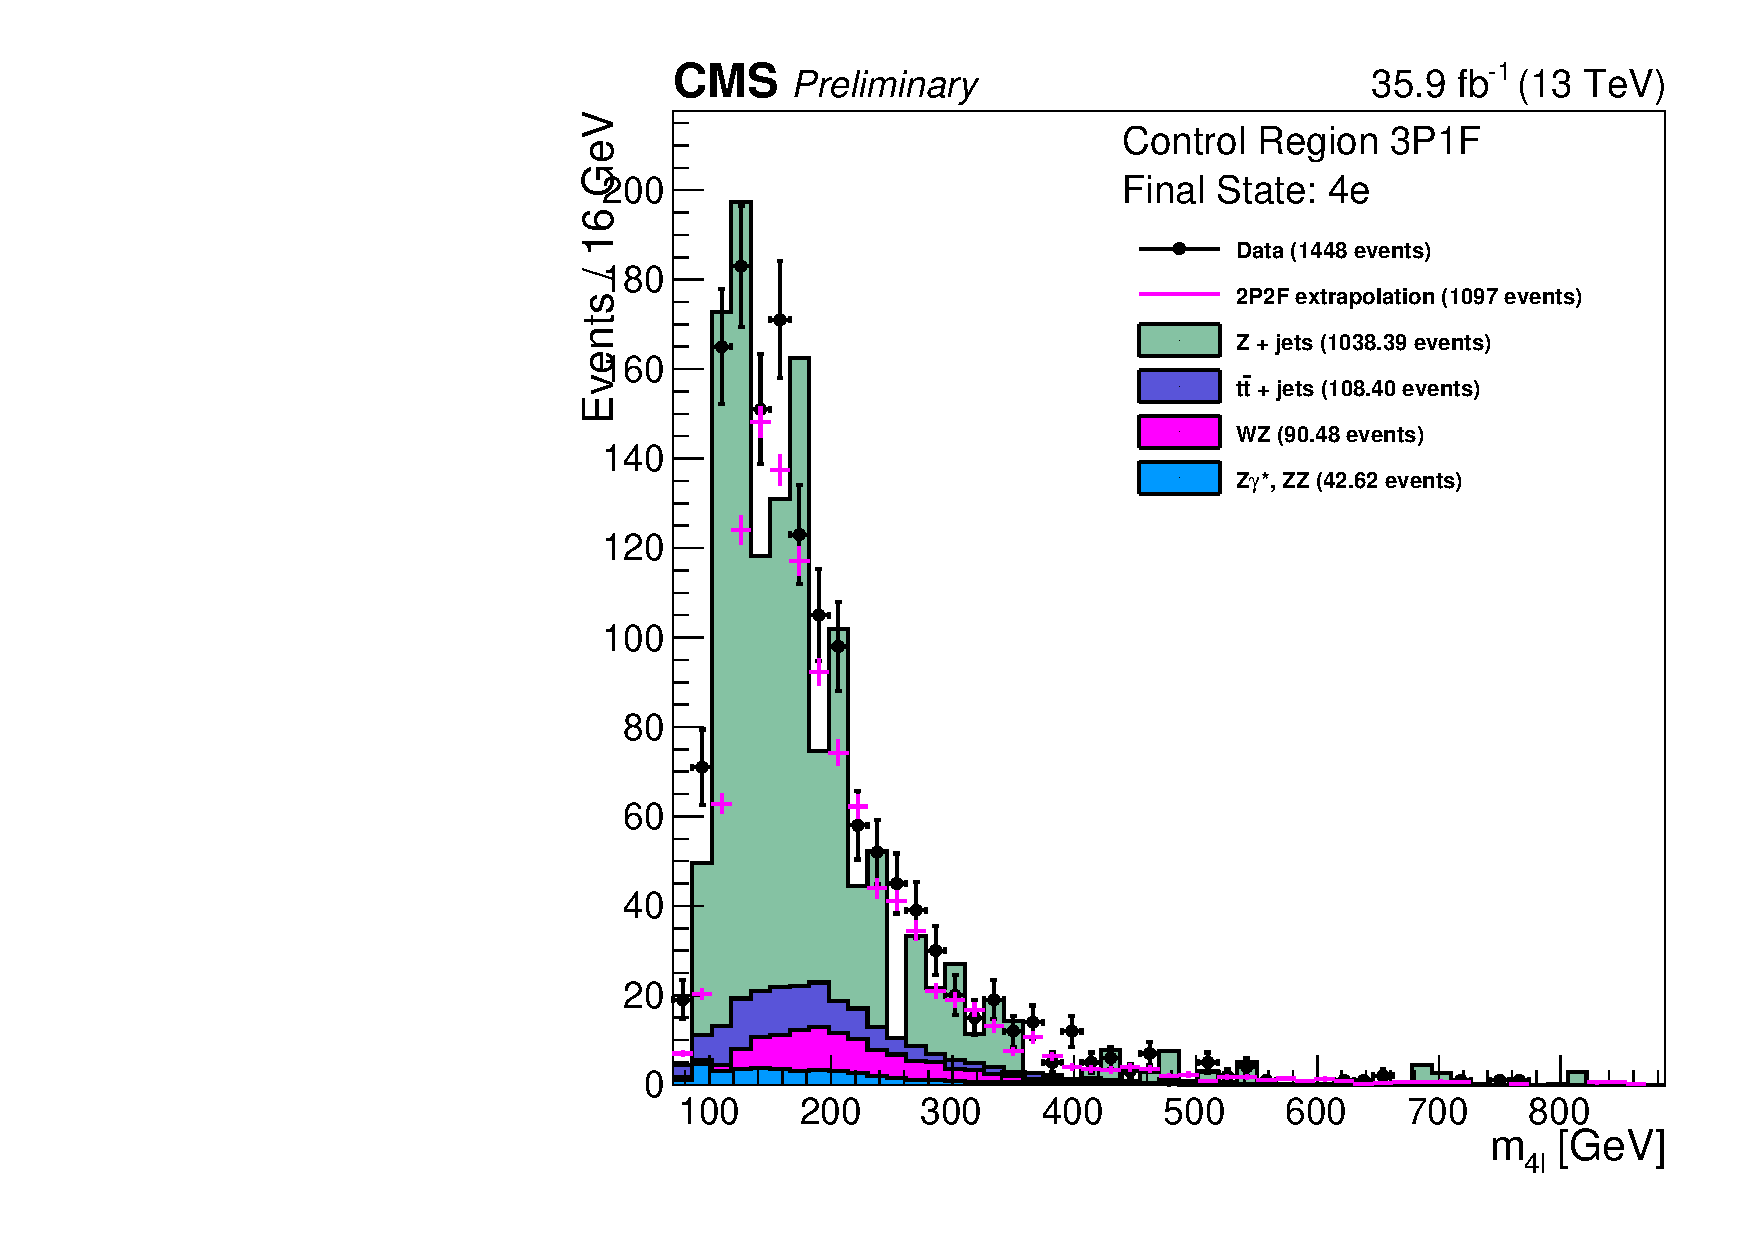
\includegraphics [width=0.45\textwidth] {Figures/RedBkg/HZZ_3P1Fuw_ZZMass_4e.pdf}} \\
    {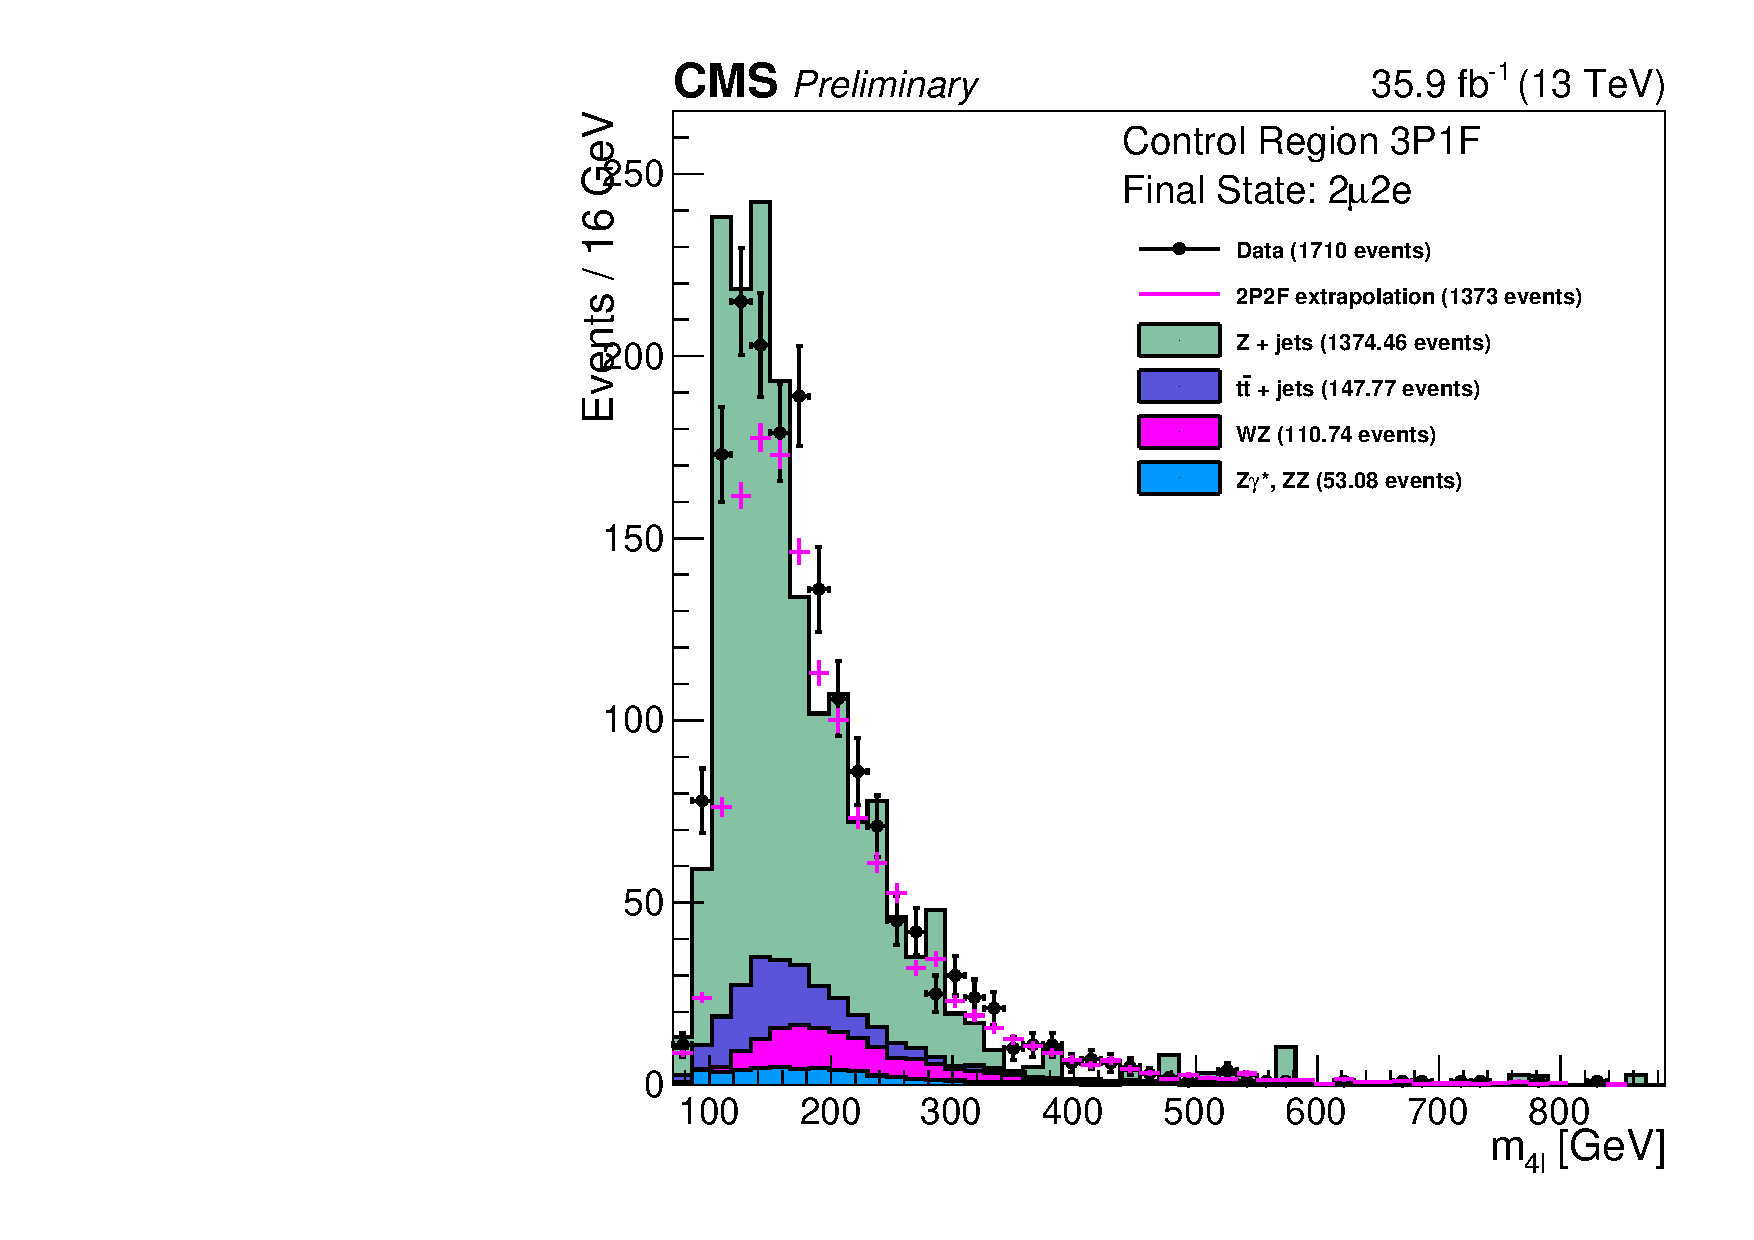
\includegraphics [width=0.45\textwidth] {Figures/RedBkg/HZZ_3P1Fuw_ZZMass_2m2e.pdf}}
    {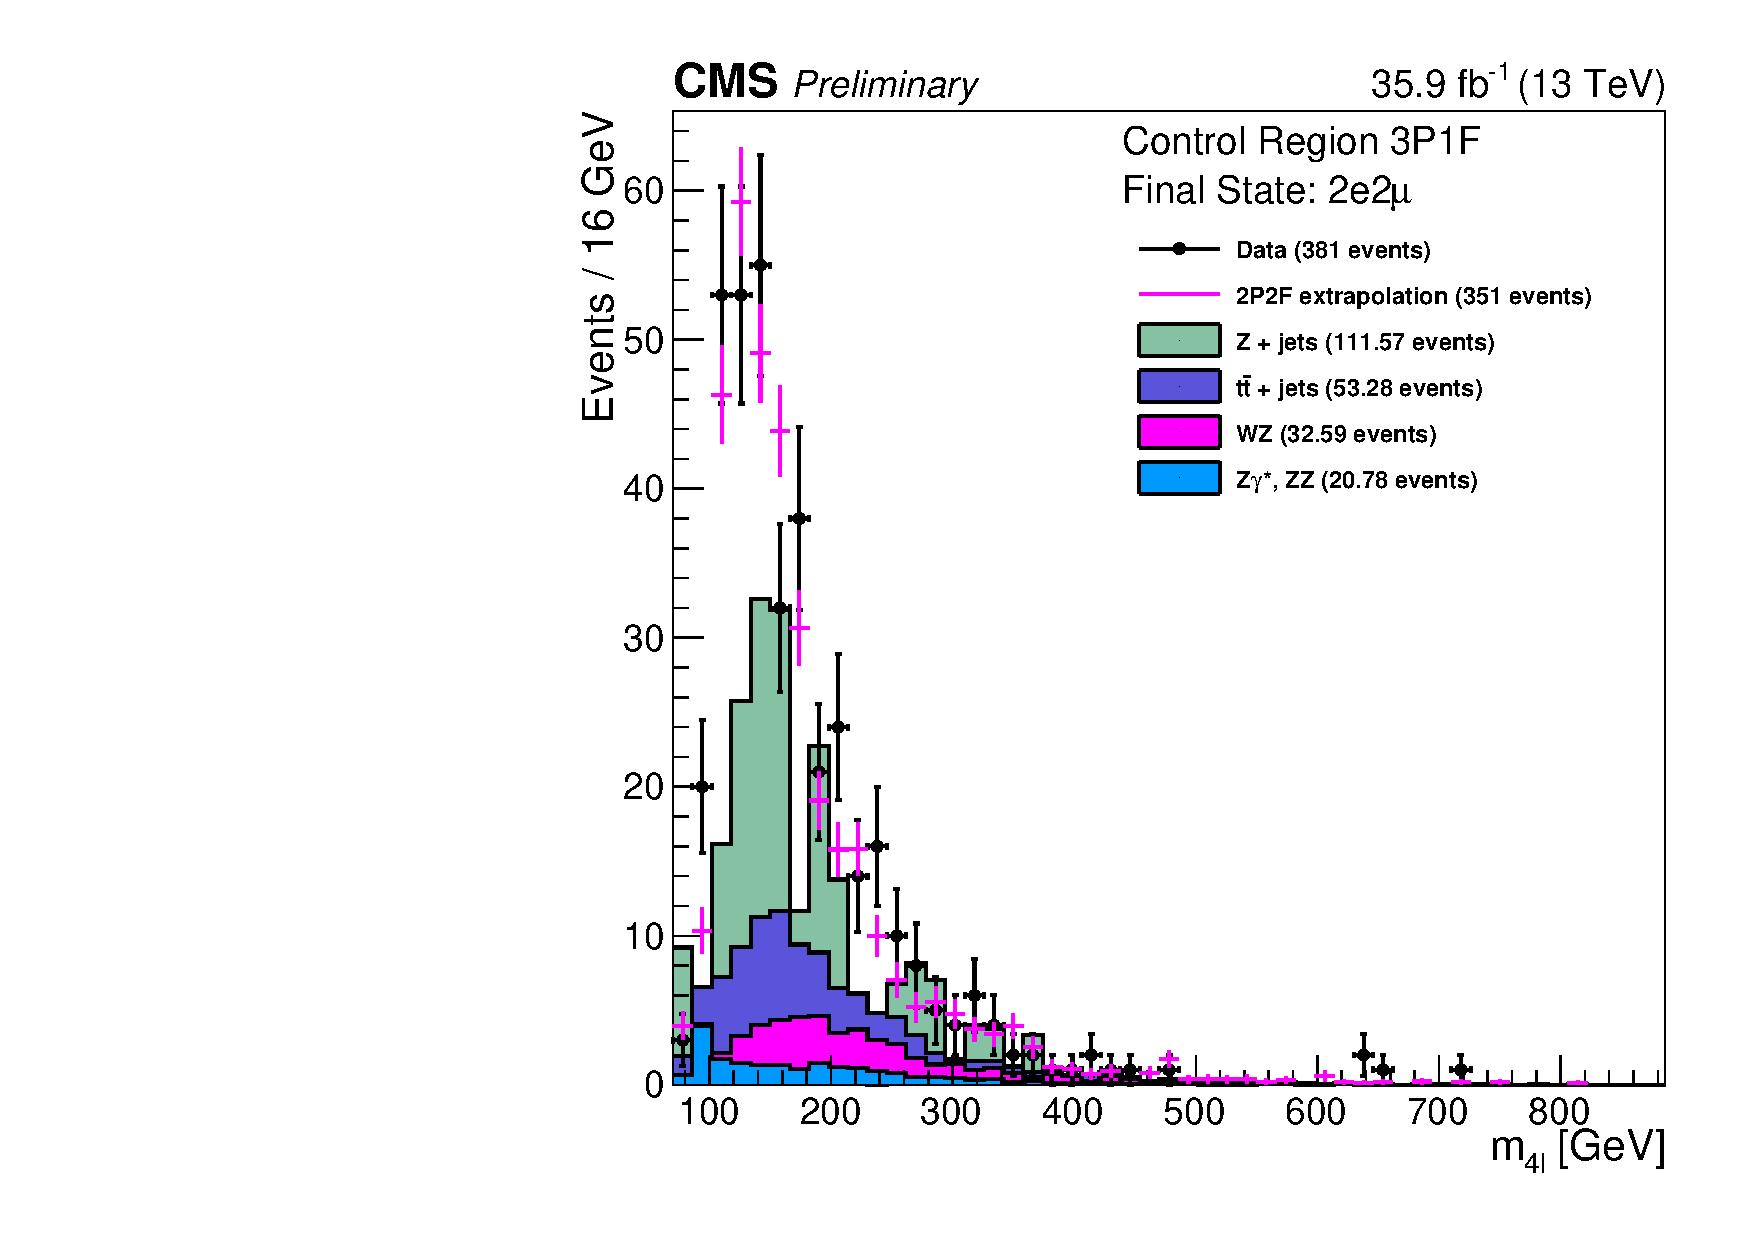
\includegraphics [width=0.45\textwidth] {Figures/RedBkg/HZZ_3P1Fuw_ZZMass_2e2m.pdf}} \\
\caption{
Invariant mass distribution of the events selected in the 3P+1F control sample in the
$13$~TeV dataset, (top left)  $4\mu$ , (top right) $4e$ , (bottom left)  $2\mu2e$ and (bottom right)  $2e2\mu$ channels.
}
\label{fig:CR_3P1F}
\end{center}
\end{figure}

The expected number of reducible background events in the 3P+1F region,
$N^{\rm bkg}_{\rm 3P1F}$, can be computed from the number of events
observed in the 2P+2F control region, $N_{\rm 2P2F}$, by weighting each
event in the region with the factor $(\frac{f_{i}}{1-f_{i}}
+ \frac{f_{j}}{1-f_{j}})$, where $f_{i}$ and $f_{j}$ correspond to the
fake ratios of the two loose leptons:

\begin{equation} 
\label{eq:Prediction3P1F}
N^{\rm bkg}_{\rm 3P1F} = \sum (\frac{f_{i}}{1-f_{i}}
+ \frac{f_{j}}{1-f_{j}}) N_{\rm 2P2F}
\end{equation} 

Figure~\ref{fig:CR_3P1F} shows the invariant mass distributions of the
events selected in the 3P+1F control sample, together with the expected
reducible background estimated from Eq.~\ref{eq:Prediction3P1F},
stacked on the distribution
of $WZ$ and of irreducible background ($ZZ, Z\gamma* \to 4\ell$) taken from the simulation.

Would the fake rates be measured in a sample that has exactly the same
background composition as the 2P+2F sample, the difference between the
observed number of events in the 3P+1F sample and the expected background
predicted from the 2P+2F sample would solely amount to the (small) $WZ$ and $Z\gamma_{conv}$
contribution. Large differences arise because the fake rates used in
Eq.~\ref{eq:Prediction3P1F} do not properly account for the background
composition of the 2P+2F control sample.


In particular, the  difference seen in Fig.~\ref{fig:CR_3P1F} between the observed
3P+1F distribution and the expectation from 2P+2F, in the
channels with loose electrons ($4e$ and $2\mu 2e$), and concentrated at low
masses, is due to photon conversions. This is confirmed explicitly by the
simulation.
% : Fig.~\ref{fig:CR_3P1F}c shows how events with a real photon populate
% this low mass region. Indeed, as the fake rates of method A are measured
% in a sample that is largely devoid of photon conversions, Eq.~\ref{eq:Prediction3P1F}
% considerably underestimates their contribution to the 3P+1F sample. 
%
The difference between the 3P+1F observation and the prediction
from 2P+2F to recover the missing contribution from conversions - and more generally,
in principle, to ``correct" for the fact that the fake rates do not properly
account for the background composition of the 2P+2F sample.
More precisely, the expected reducible background in the signal region is given
by the sum of two terms :
%
\begin{itemize}
\item a ``2P2F component", obtained from the number of
  events observed in the 2P+2F control region, $N_{\rm 2P2F}$, by
  weighting each event in that region with the factor
  $\frac{f_{i}}{1-f_{i}} \frac{f_{j}}{1-f_{j}}$, where $f_{i}$ and
  $f_{j}$ correspond to the fake ratios of the two loose leptons.
\item a ``3P1F component", obtained from the
   difference between the number of observed events in the 3P+1F control
   region, $N_{\rm 3P1F}$, and the expected contribution from the 2P+2F
   region and ZZ processes in the signal region, $N^{\rm ZZ}_{\rm 3P1F} +
   N^{\rm bkg}_{\rm 3P1F}$. The $N^{\rm bkg}_{\rm 3P1F}$ is given by 
   equation \ref{eq:Prediction3P1F} and $N^{\rm ZZ}_{\rm 3P1F}$ is the
   contribution from $ZZ$ which is taken from the simulation. 
   The difference $N_{\rm 3P1F} -  N^{\rm bkg}_{\rm 3P1F} - N^{\rm ZZ}_{\rm 3P1F}$,
   which may be negative,
   is obtained for each $(p_T, \eta)$ bin of the ``F" lepton, and is weighted 
   by $\frac{f_i} {1 - f_i}$, where $f_i$ denotes the fake rate of
   this lepton.
   This ``3P1F component" accounts for the contribution of reducible background
   processes with only one fake lepton (like $WZ$ events), and for the contribution
   of other processes (e.g. photon conversions) that are not properly estimated
   by the 2P2F component, because of the fake rates used.
\end{itemize}

Therefore, the
full expression for the prediction can be symbolically written as:
%
\begin{equation} 
\label{eq:PredictionSR}
N^{bkg}_{\rm SR} = \sum \frac{f_{i}}{(1-f_{i})} (N_{\rm 3P1F} - N^{\rm
bkg}_{\rm 3P1F} - N^{\rm ZZ}_{\rm 3P1F})
+ \sum \frac{f_{i}}{(1-f_{i})} \frac{f_{j}}{(1-f_{j})}N_{\rm 2P2F} \end{equation}
%a
Previous equation is equivalent to the following:
\begin{equation}
\label{eq:PredictionSR2}
N^{bkg}_{\rm SR}= (1-\frac{N_{3P1F}^{ZZ}}{N_{3P1F}})\sum_j^{N_{3P1F}}\frac{f_a^j}{1-f_a^j} - \sum_i^{N_{2P2F}}\frac{f_3^i}{1-f_3^i}\frac{f_4^i}{1-f_4^i}
\end{equation}
For channels where the $Z_2$ candidate is made from two electrons, 
the contribution of the 3P1F component is 
positive, and amounts to typically $30 \%$ of the total predicted background.

For channels with loose muons ($4\mu$ and $2e2\mu$), the 3P+1F sample is rather well described by
the prediction from 2P+2F, as seen in Fig.~\ref{fig:CR_3P1F}b, and the
3P1F component is mainly driven by statistical fluctuations in the 3P+1F sample,
which are larger than the expectation from $WZ$ production.


Table~\ref{tab:reducibleMethodA} shows the expected number of
events in the signal regions from the reducible background processes for the 13 TeV. 
% The first error is the statistical uncertainty, which is dominated by the
% large statistical uncertainty of the ``3P1F" component. The second error
% is a systematic uncertainty due to the statistical uncertainty of the
% fake rates.

\begin{table}[h]
\begin{center}
     \begin{tabular}{| l | c | c | c | c |} \hline
 baseline	& 4e 	 & 4$\mu$ & 2e2$\mu$  & 2$\mu$2e   \\ \hline \hline
 13 TeV		& $22.19$ & $32.81$ & $22.48$    & $41.72$  \\  \hline
 	\end{tabular}
\end{center}
    \caption{ The contribution of reducible background
    processes in the signal region predicted from measurements in data
    using the Opposite-Sign Leptons method. The predictions correspond to \usedLumi of data at 13 TeV.}
     \label{tab:reducibleMethodA}
\end{table}
